\documentclass[10pt,twocolumn,letterpaper]{article}
\usepackage{cite}
\usepackage{amsmath,amssymb,amsfonts}
\usepackage{amsmath,amssymb,amsfonts}
\usepackage{graphicx}
\usepackage{textcomp}
\usepackage{xcolor}
\usepackage{hyperref}
\usepackage{float}

\def\BibTeX{{\rm B\kern-.05em{\sc i\kern-.025em b}\kern-.08em
    T\kern-.1667em\lower.7ex\hbox{E}\kern-.125emX}}

\begin{document}

\title{FamineSight: Predicting Hunger-Related Mortality in Somalia Using Artificial Intelligence\\
{\large \textsuperscript{*}CSCI.720.01 - Big Data Analytics}
}

\author{Anurag Lnu \\
Rochester Institute of Technology \\
Rochester, NY \\
al5150@rit.edu}

\maketitle

\begin{abstract}
FamineSight is an end-to-end early warning system designed to predict hunger-related mortality in Somalia. It integrates an array of diverse data streams, including ACLED conflict reports, WFP food prices, CHIRPS rainfall metrics, satellite NDVI, and IPC phase classifications. By utilizing advanced machine learning and data mining techniques—such as robust classification, multivariate clustering, anomaly detection, and association rule mining—the system provides actionable warnings. This paper details the complete data mining pipeline, encompassing extensive exploratory data analysis, evaluation of various predictive models in an "Algorithm Zoo", and the architectural synthesis into a real-time humanitarian decision support system.
\end{abstract}

\textbf{Keywords:} Data Mining, Famine Early Warning, Predictive Analytics, Machine Learning, Humanitarian Tech

\section{Introduction}
Acute food insecurity and famine remain catastrophic realities in the Horn of Africa, particularly in Somalia, where prolonged droughts, economic fragility, and protracted conflict frequently converge. Traditional early warning systems often suffer from significant latency, relying on lagging indicators such as demographic anthropometric measurements that signal a crisis only after severe human toll has occurred \cite{Maxwell2015}.

FamineSight is designed to bridge this gap by deploying cutting-edge artificial intelligence over high-frequency, multi-dimensional humanitarian data streams \cite{Lentz2020}. Operating as an end-to-end analytical pipeline, FamineSight tracks real-time shifts in climatic hazards, market shocks, and social instability to forecast famine conditions months in advance. The core technical contribution lies in its comprehensive data mining architecture—encompassing sophisticated imputation, high-dimensional exploratory data analysis (EDA), predictive classification with severe class imbalance handling, density-based clustering, multi-variate anomaly detection, and frequent pattern mining.

\section{Data Sourcing and Preprocessing}
The success of FamineSight relies on synthesizing nine disparate data sources into a unified district-month spatio-temporal panel.

\subsection{Data Sources}
The foundation dataset incorporates:
\begin{itemize}
    \item \textbf{ACLED}: Conflict events, civilian targeting, and fatalities \cite{Raleigh2010}.
    \item \textbf{WFP}: Macroeconomic indicators and local food market prices.
    \item \textbf{CHIRPS}: Gridded precipitation anomaly data \cite{Funk2015}.
    \item \textbf{NDVI}: Satellite-derived vegetation health indices.
    \item \textbf{UNHCR \& IOM}: Internal displacement records.
    \item \textbf{IPC \& FSNAU}: Ground-truth Integrated Food Security Phase Classifications and crude death rates.
\end{itemize}

\subsection{Data Quality and Imputation}
Real-world humanitarian datasets exhibit severe sparseness, noise, and irregularity. Missingness was evaluated prior to imputation (Figure \ref{fig:missing_pct}). Features with excessive gaps necessitated robust techniques such as K-Nearest Neighbors (KNN) imputation \cite{Little2019} to preserve the underlying localized feature structures, while interpolation was used for temporal continuity.

\begin{figure}[H]
    \centering
    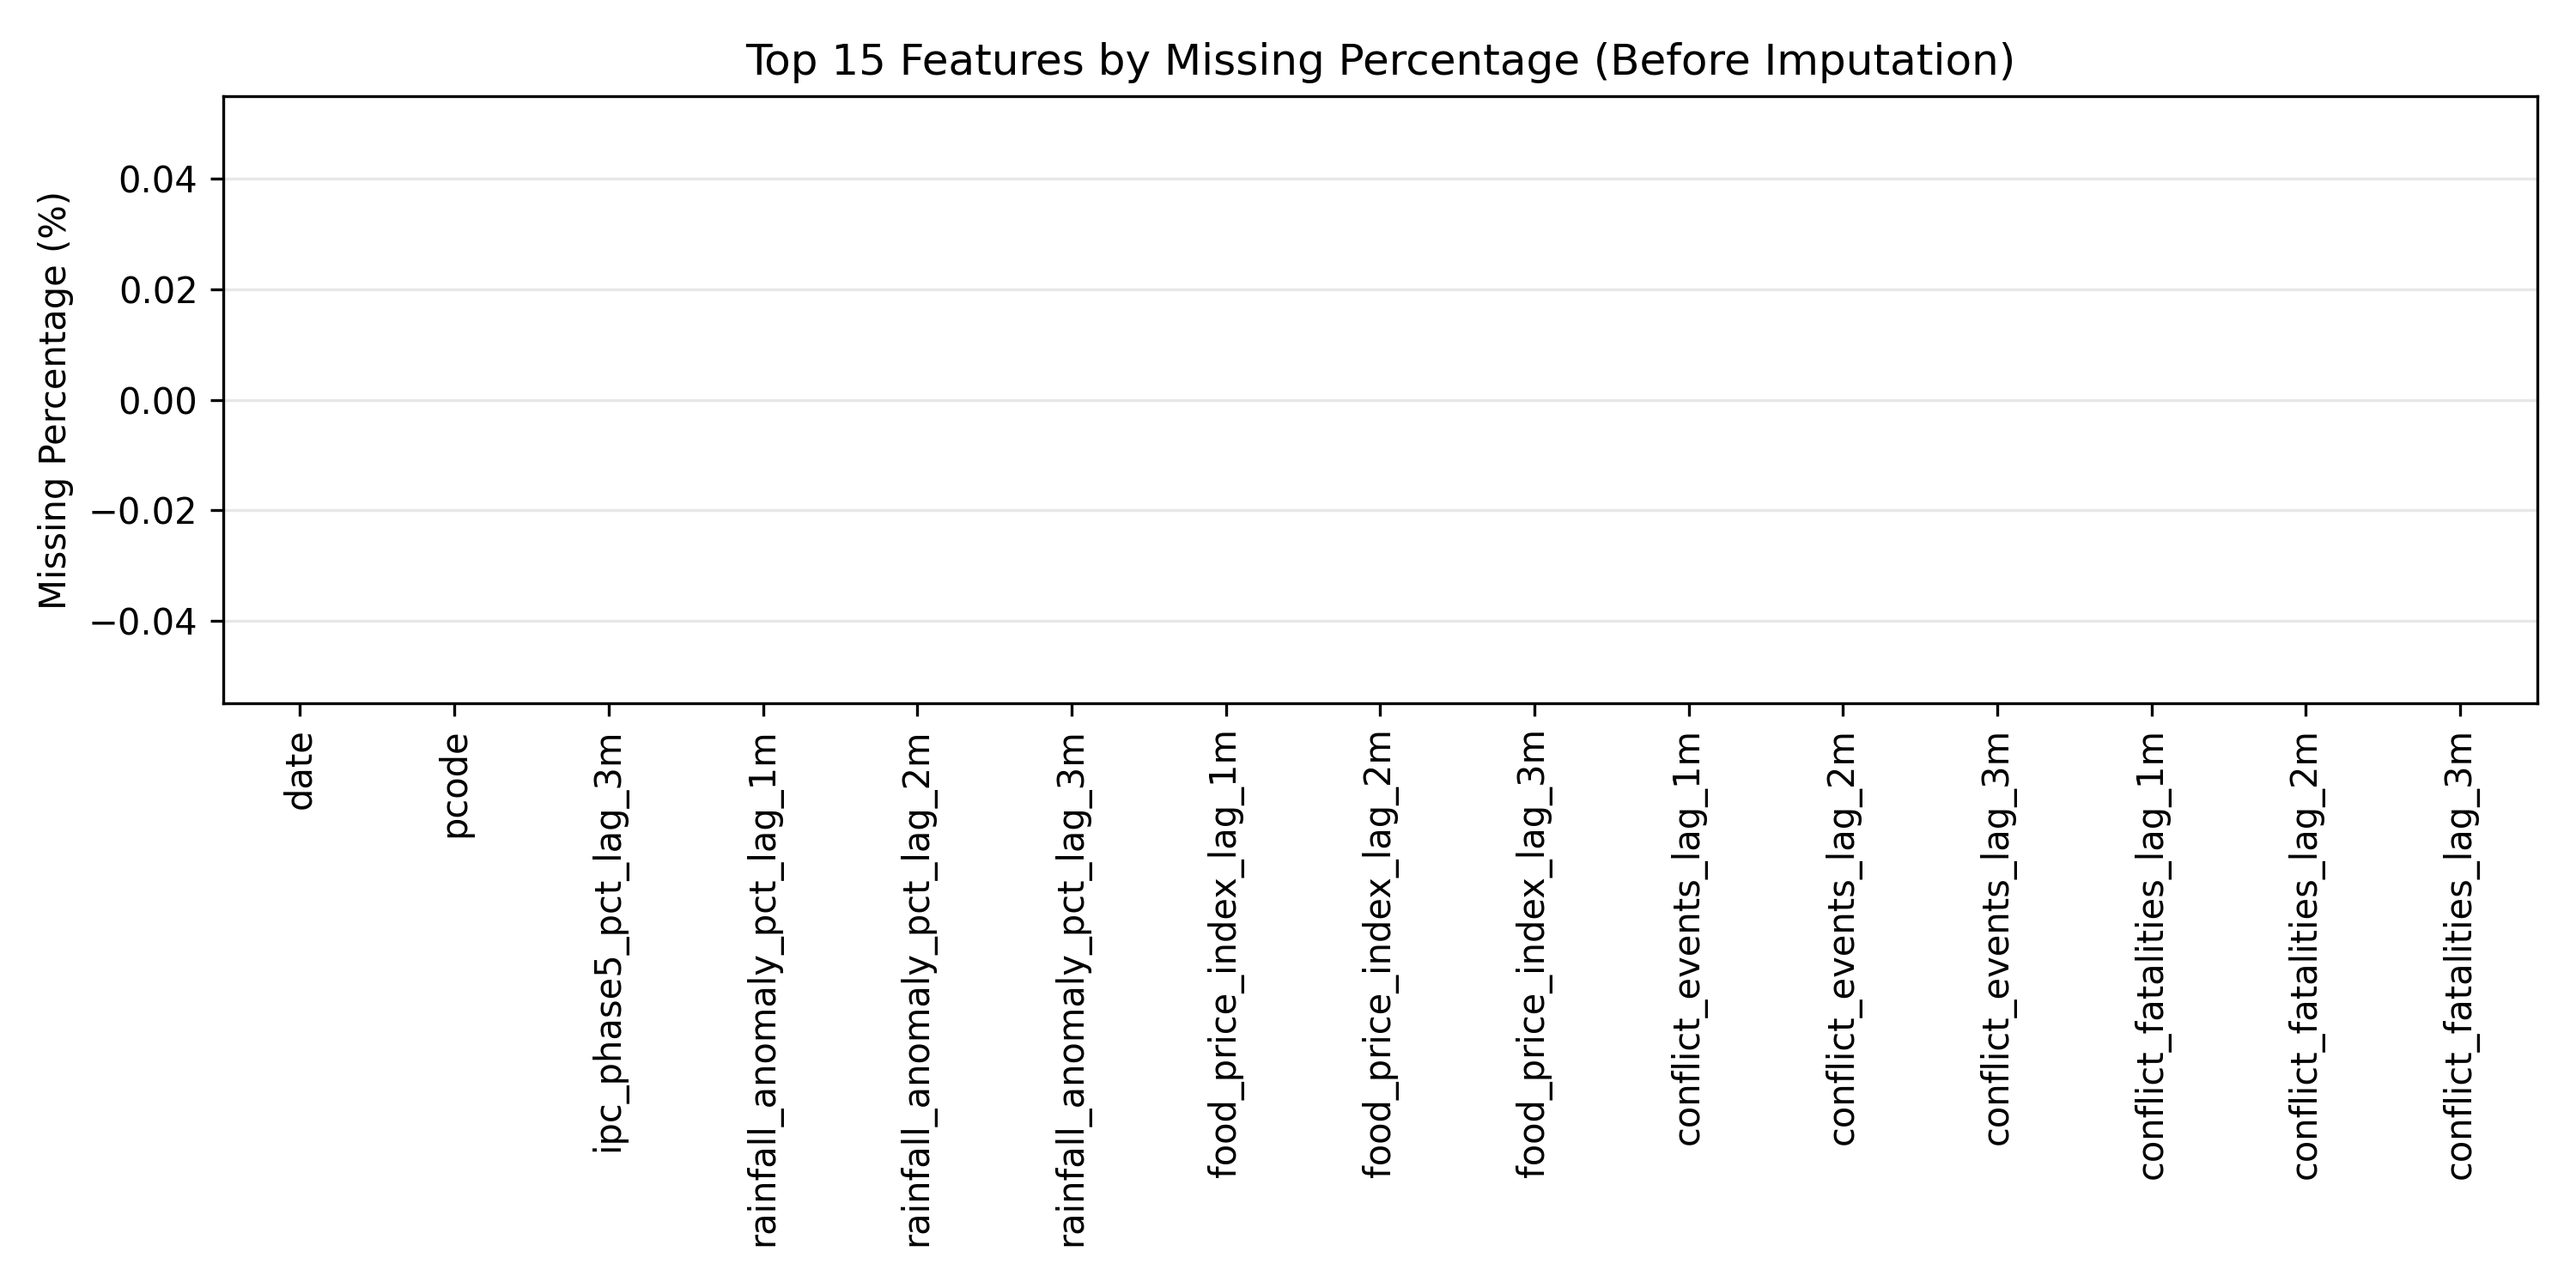
\includegraphics[width=0.48\textwidth]{figures/missing_pct.png}
    \caption{Top 15 features ranked by missing data percentages prior to systematic imputation.}
    \label{fig:missing_pct}
\end{figure}

The distribution of outliers was quantified using Z-score boundaries ($Z > 3$), highlighting the volatile, heavy-tailed nature of the underlying data (Figure \ref{fig:outlier_pct}). Such skewed distributions dictated the application of robust scaling methodologies (e.g., MinMax and robust scalers) to ensure stable convergence in distance-based modeling like K-Means.

\begin{figure}[H]
    \centering
    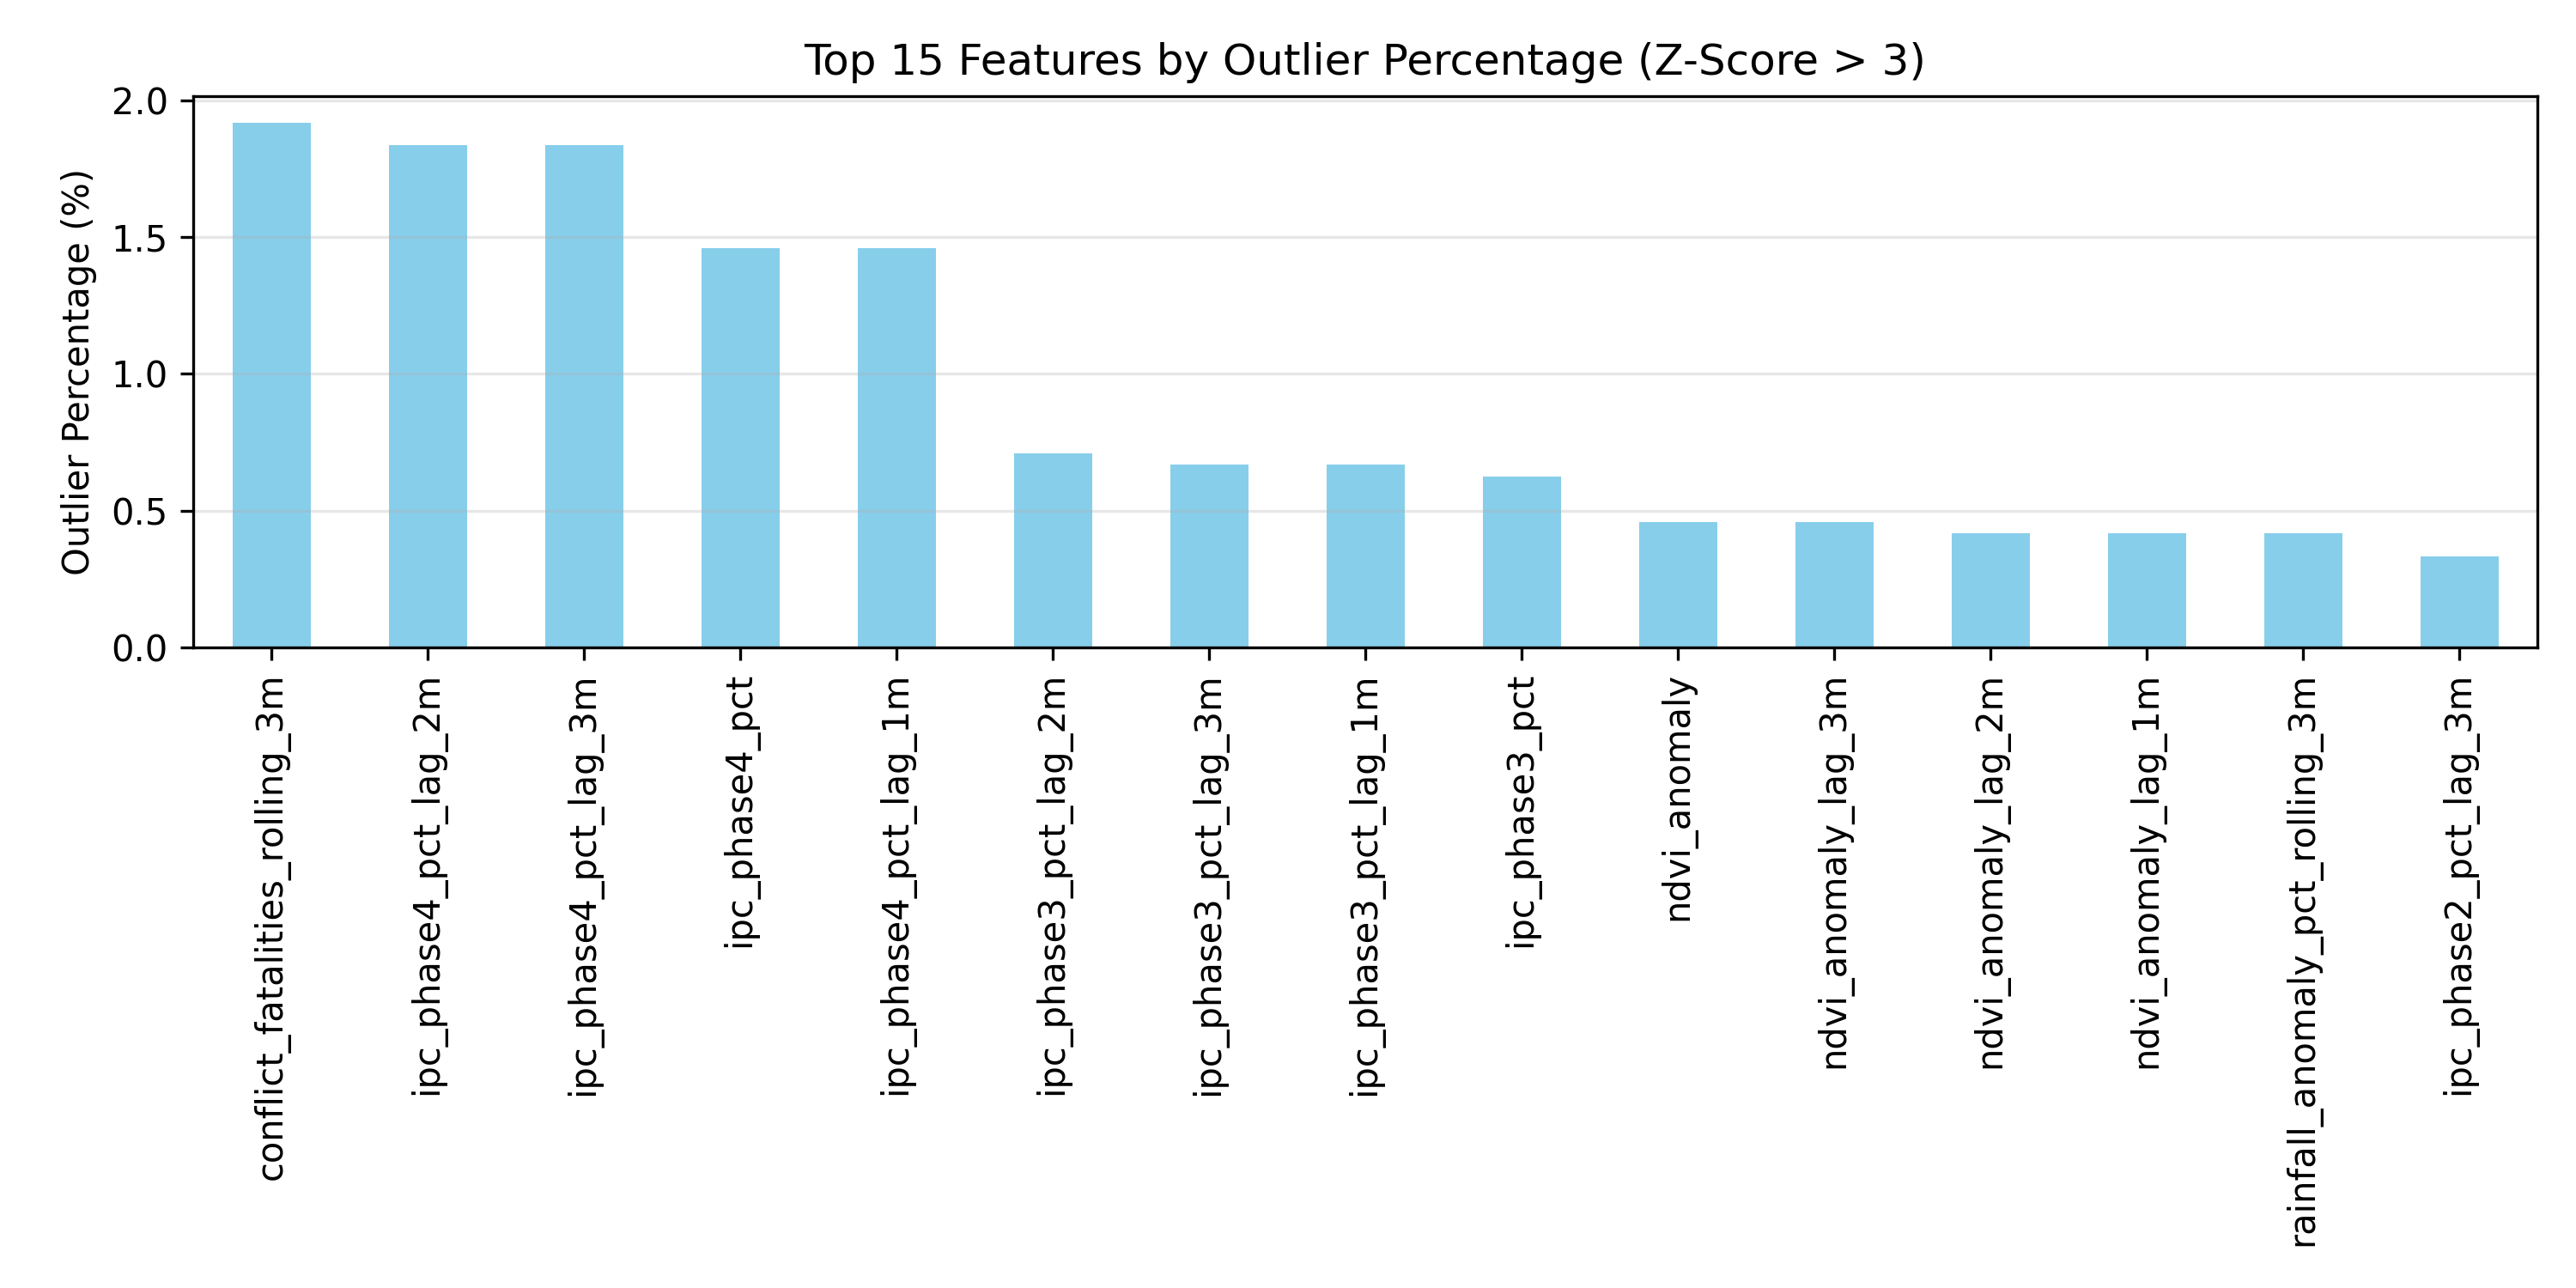
\includegraphics[width=0.48\textwidth]{figures/outlier_pct.png}
    \caption{Outlier frequency indicating the heavy-tailed, bursty nature of crisis events and market shocks.}
    \label{fig:outlier_pct}
\end{figure}

\subsection{Feature Engineering}
Engineering temporal awareness was paramount. The pipeline calculated rolling windows and temporal lags (1-to-3 months) for core metrics like precipitation and conflict fatalities. Autocorrelation analysis (Figure \ref{fig:lag_autocorr}) confirmed the persistent effect of lagged environmental stressors.

\begin{figure}[H]
    \centering
    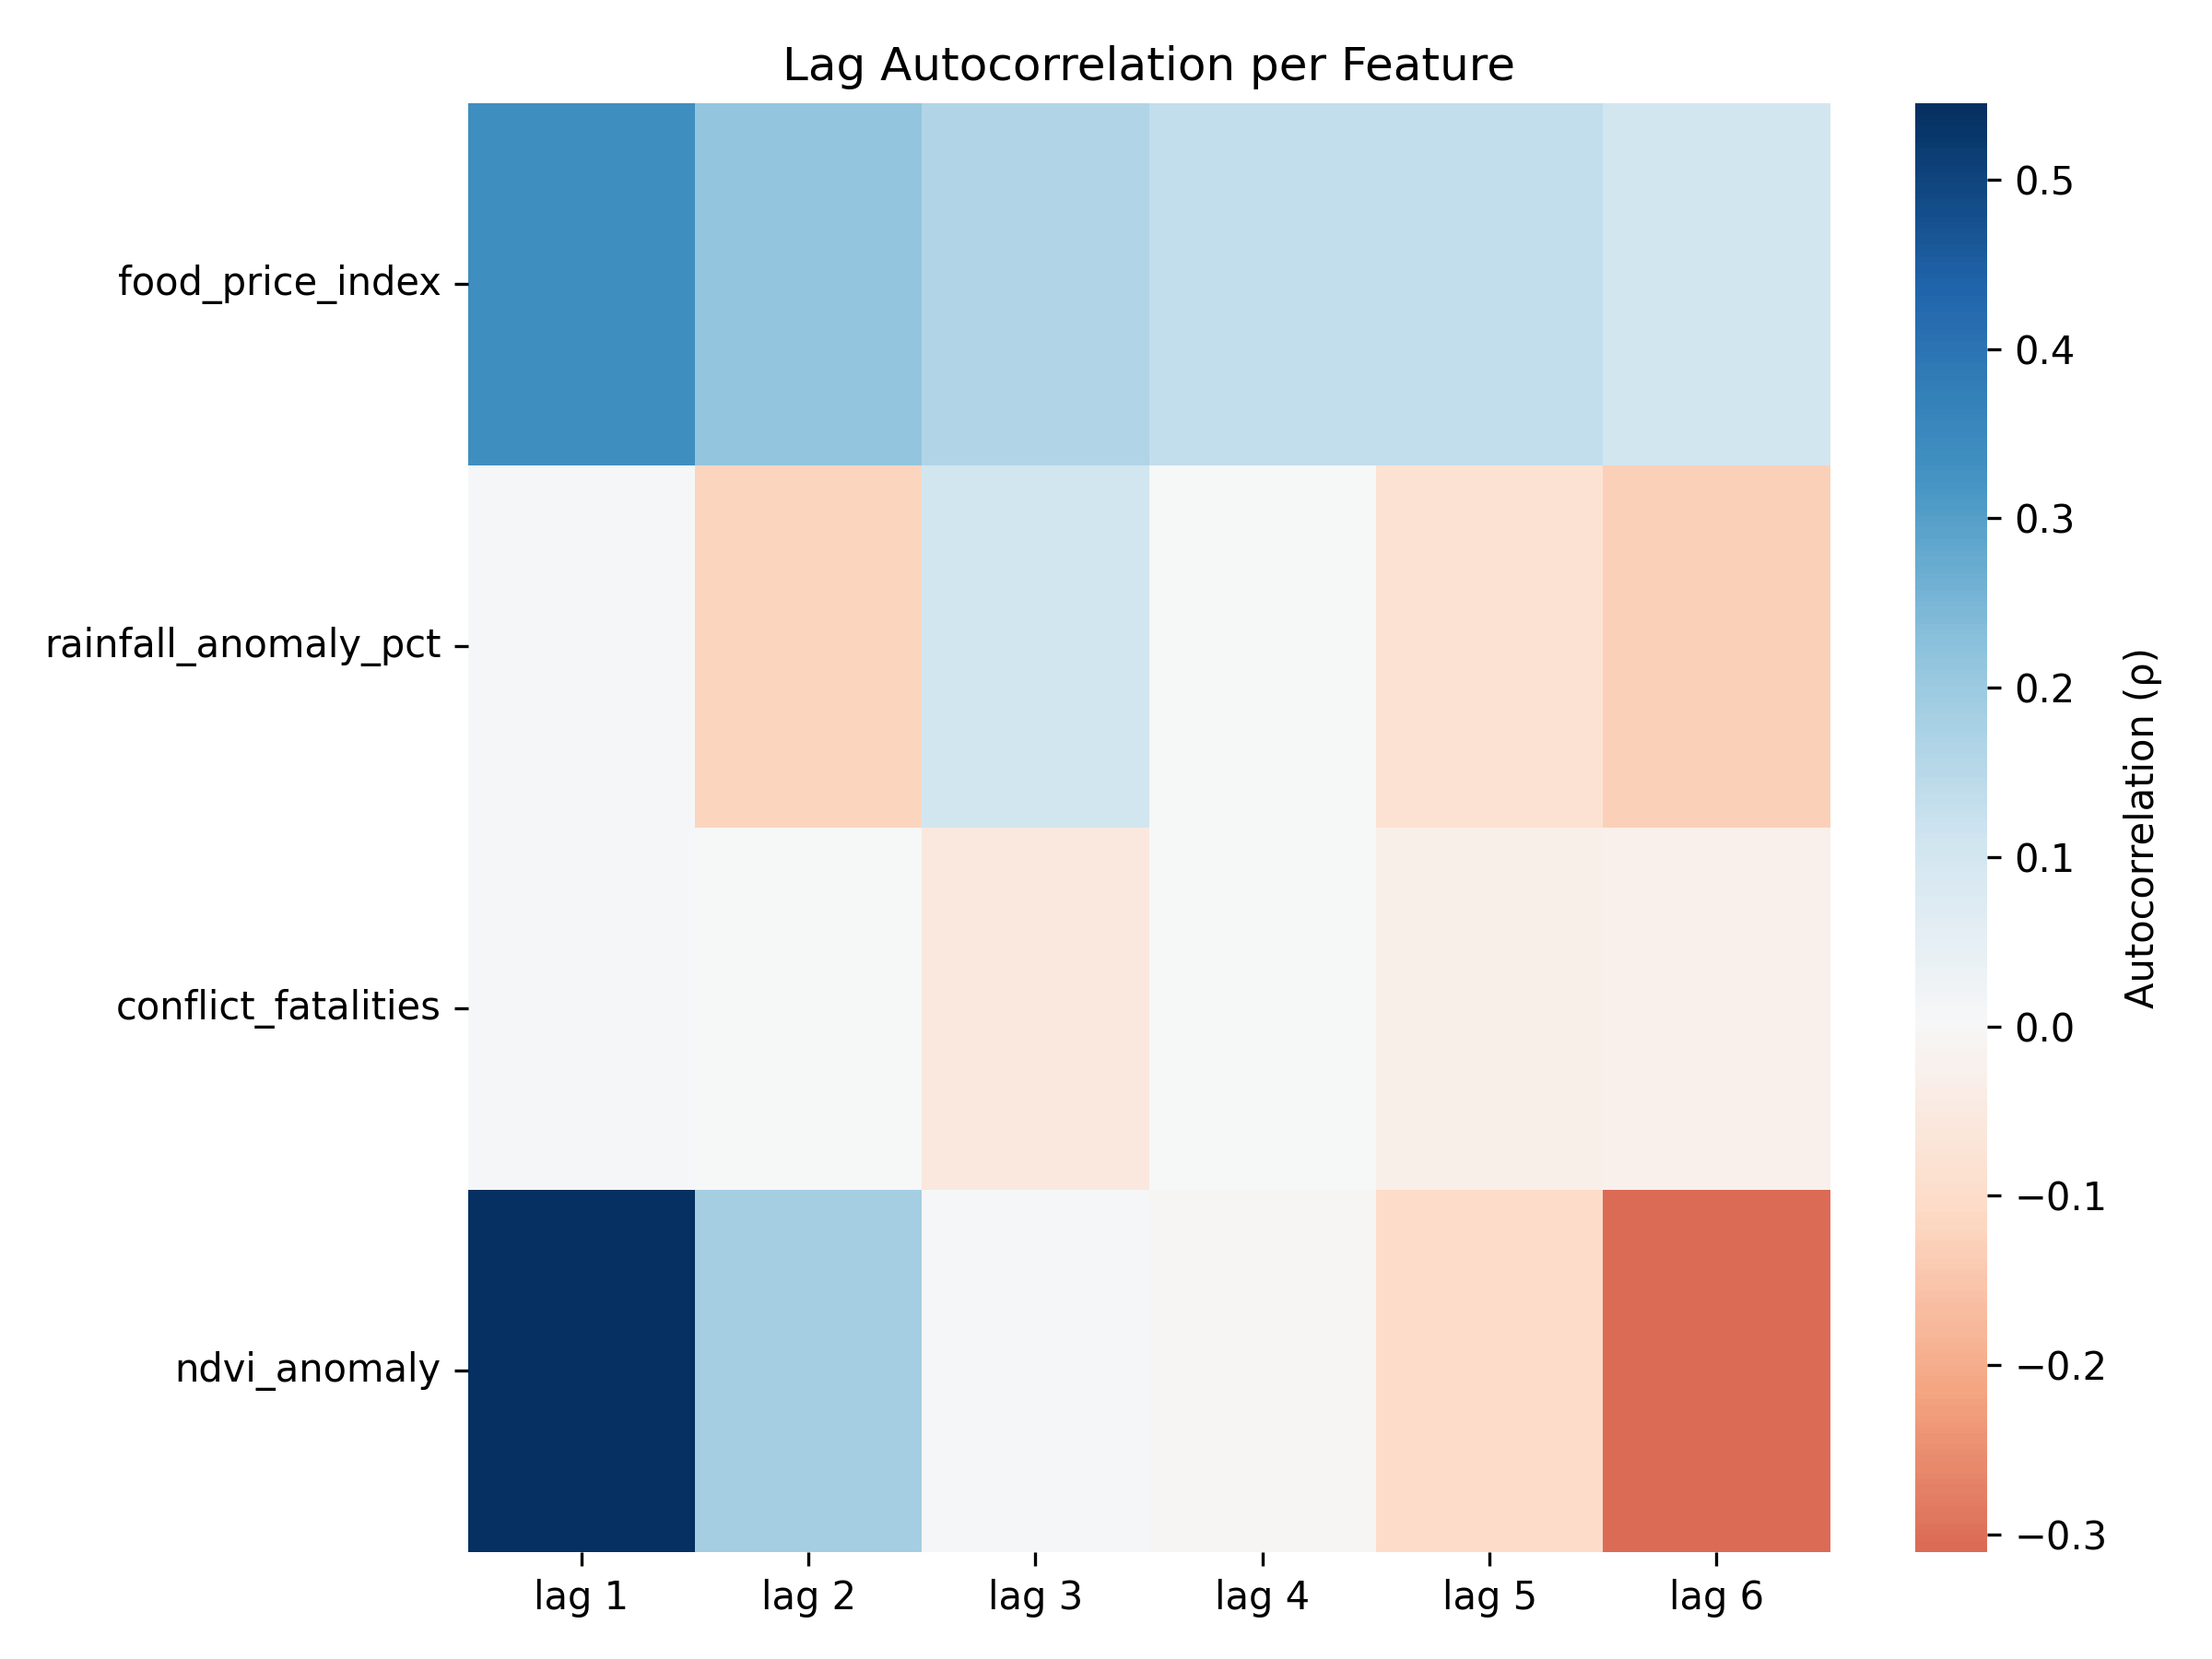
\includegraphics[width=0.48\textwidth]{figures/lag_autocorr.png}
    \caption{Autocorrelation matrix visualizing the temporal persistence of indicators across varying lag periods.}
    \label{fig:lag_autocorr}
\end{figure}

Extensive feature selection was validated using Chi-Square ($\chi^2$) and Mutual Information scores to prune uninformative features and reduce dimensionality (Figure \ref{fig:feature_selection}).

\begin{figure}[H]
    \centering
    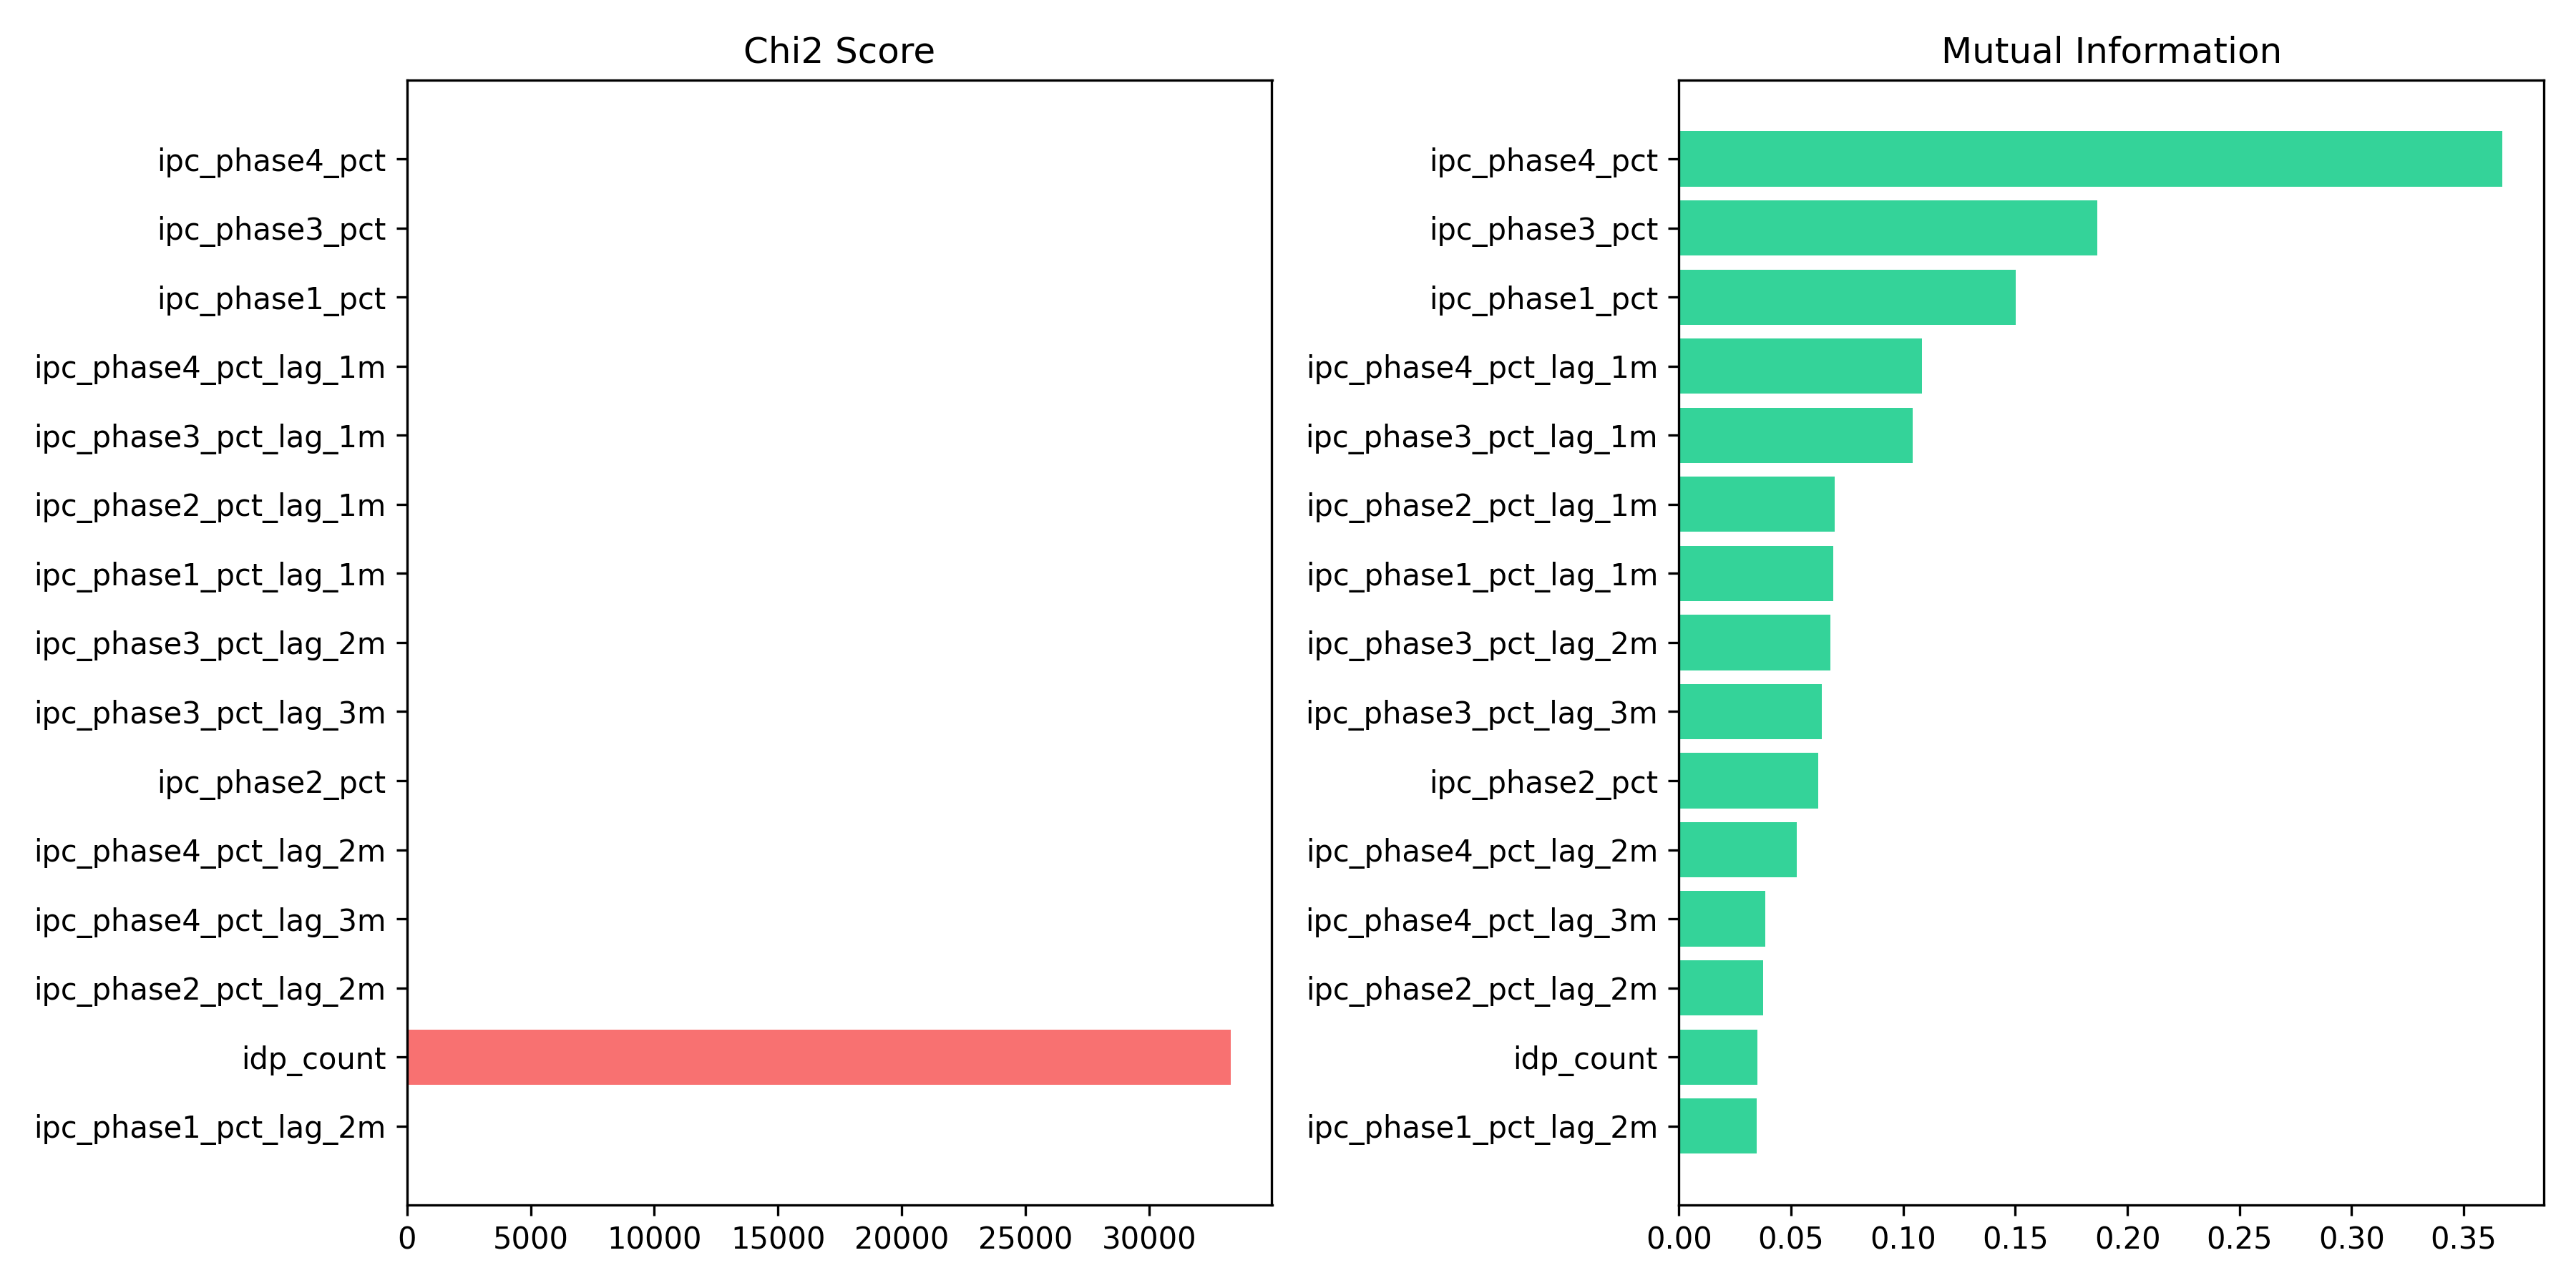
\includegraphics[width=0.48\textwidth]{figures/feature_selection.png}
    \caption{Feature ranking using Chi-Square (left) and Mutual Information (right), identifying optimal predictors for the downstream classification.}
    \label{fig:feature_selection}
\end{figure}

\section{Exploratory Data Analysis (EDA)}
EDA uncovered the macro-level behavior of Somalia's humanitarian landscape. As seen in Figure \ref{fig:crisis_trend}, the temporal accumulation of crises explicitly mirrors historical tragedy periods, notably the 2011 and 2017 famines.

\begin{figure}[H]
    \centering
    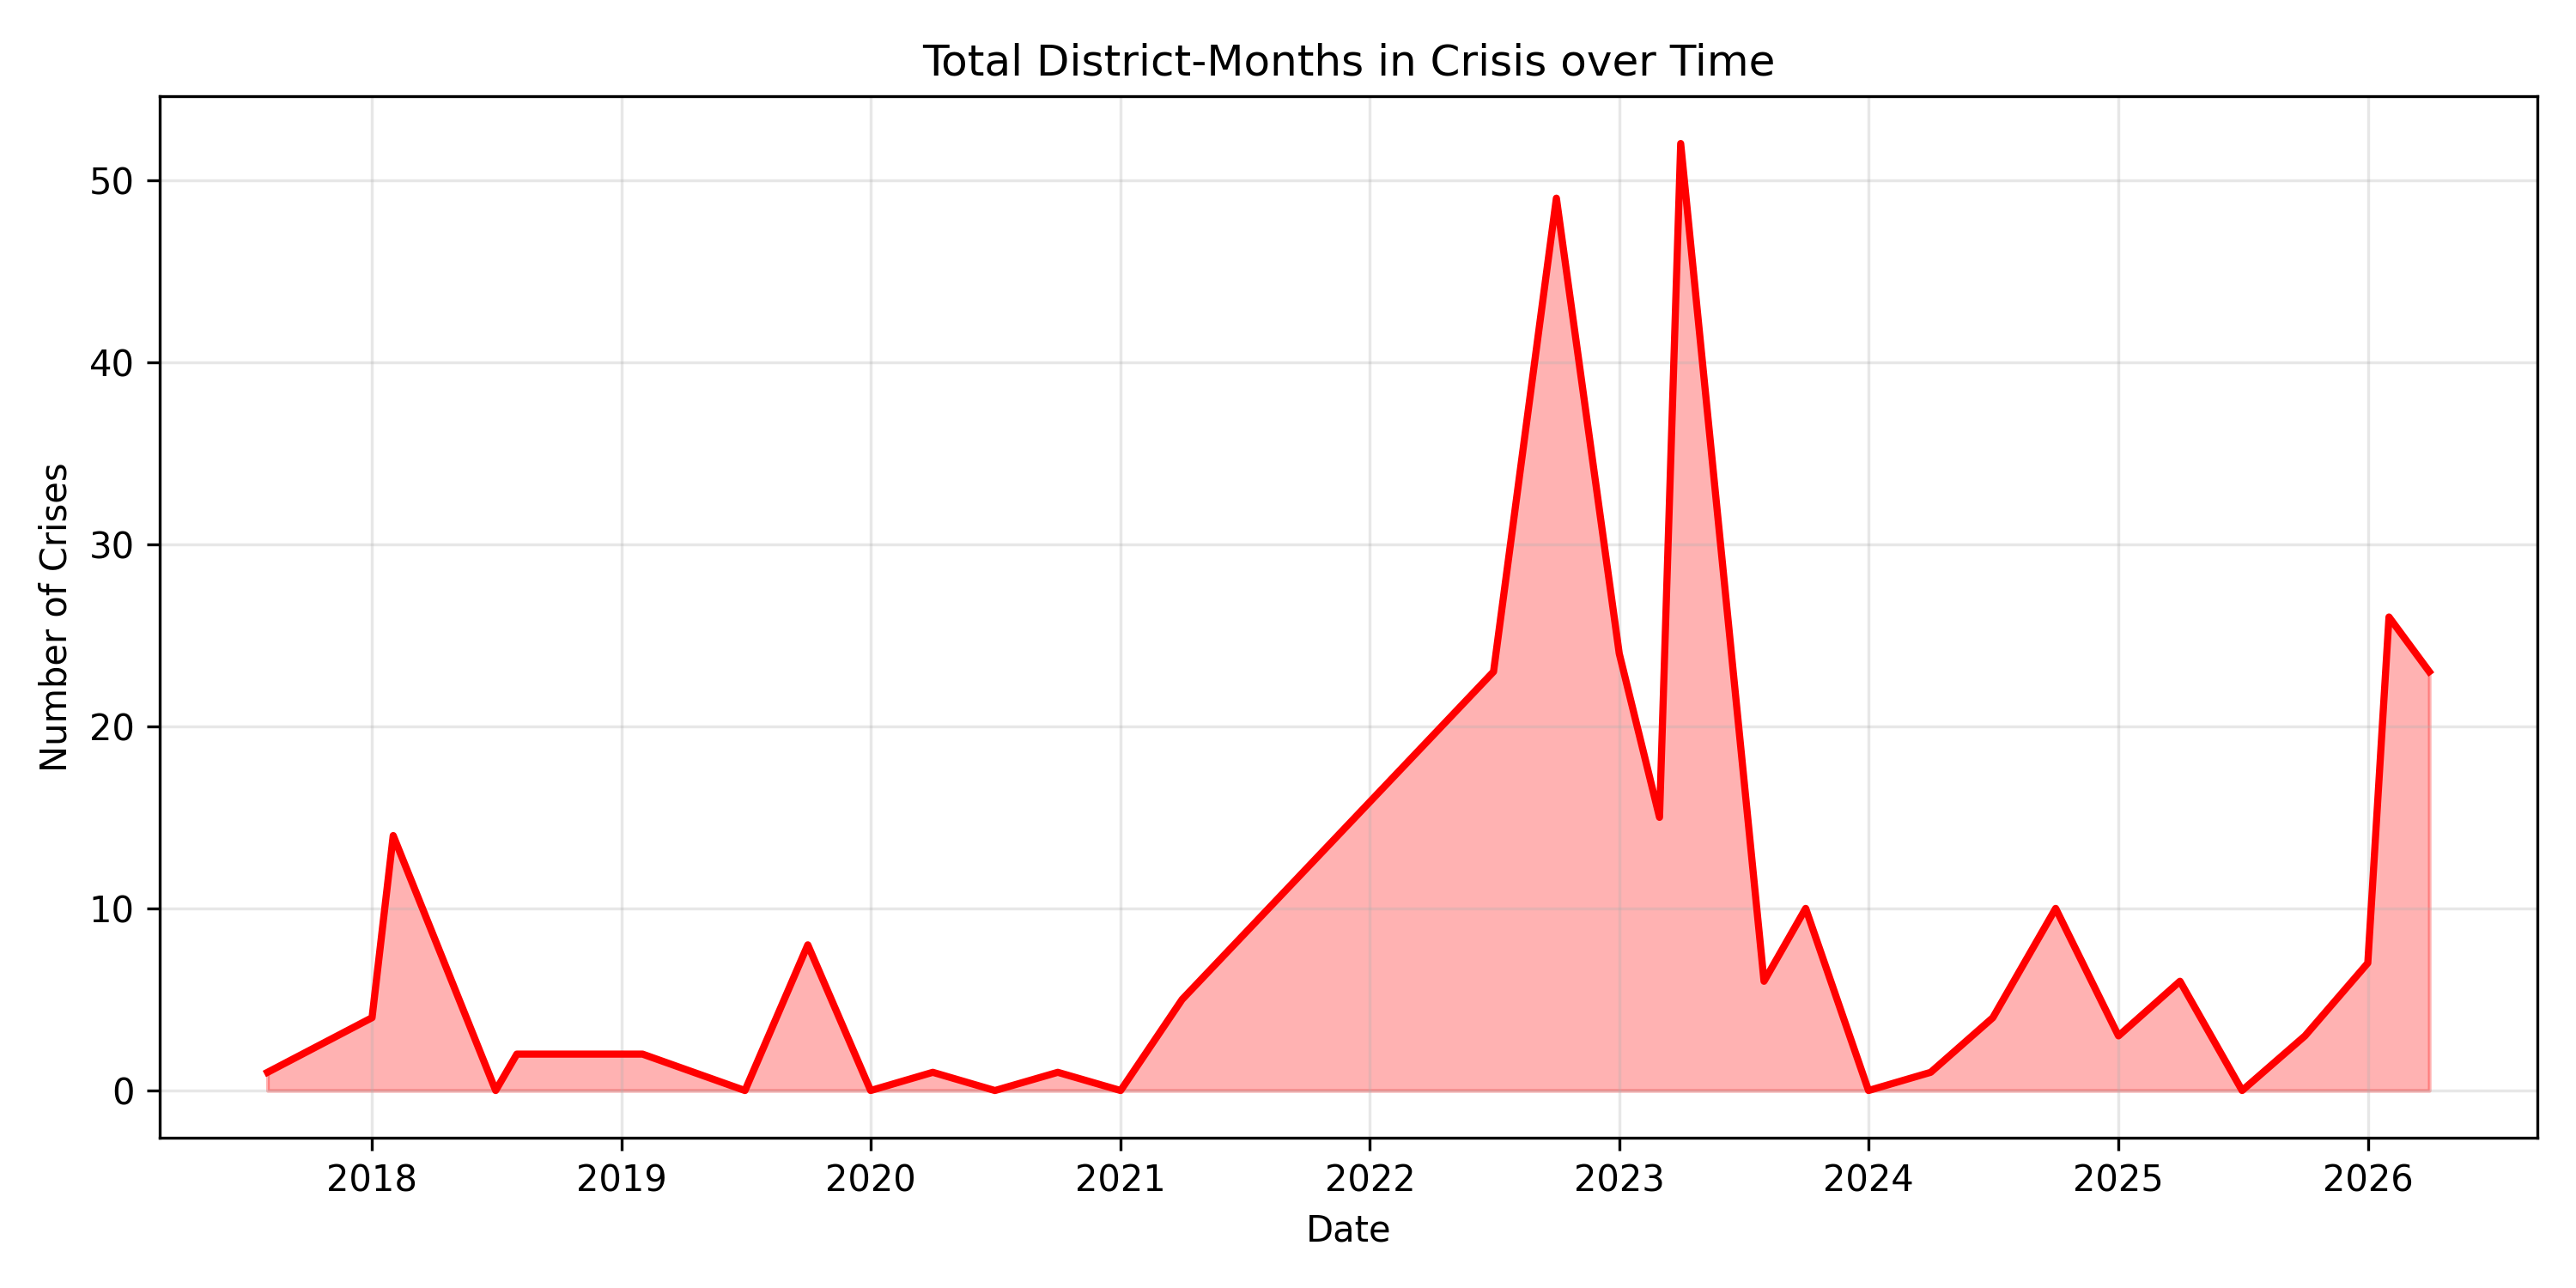
\includegraphics[width=0.48\textwidth]{figures/crisis_trend.png}
    \caption{Time-series footprint of district-months labeled as crisis, illustrating periodic systemic distress across the region.}
    \label{fig:crisis_trend}
\end{figure}

\subsection{Correlations and Distributions}
Correlation mapping (Figure \ref{fig:correlation_heatmap}) reinforced domain hypotheses, highlighting strong multi-collinearity between rolling conflict averages, severe negative rainfall anomalies, and escalating local food prices.

\begin{figure}[H]
    \centering
    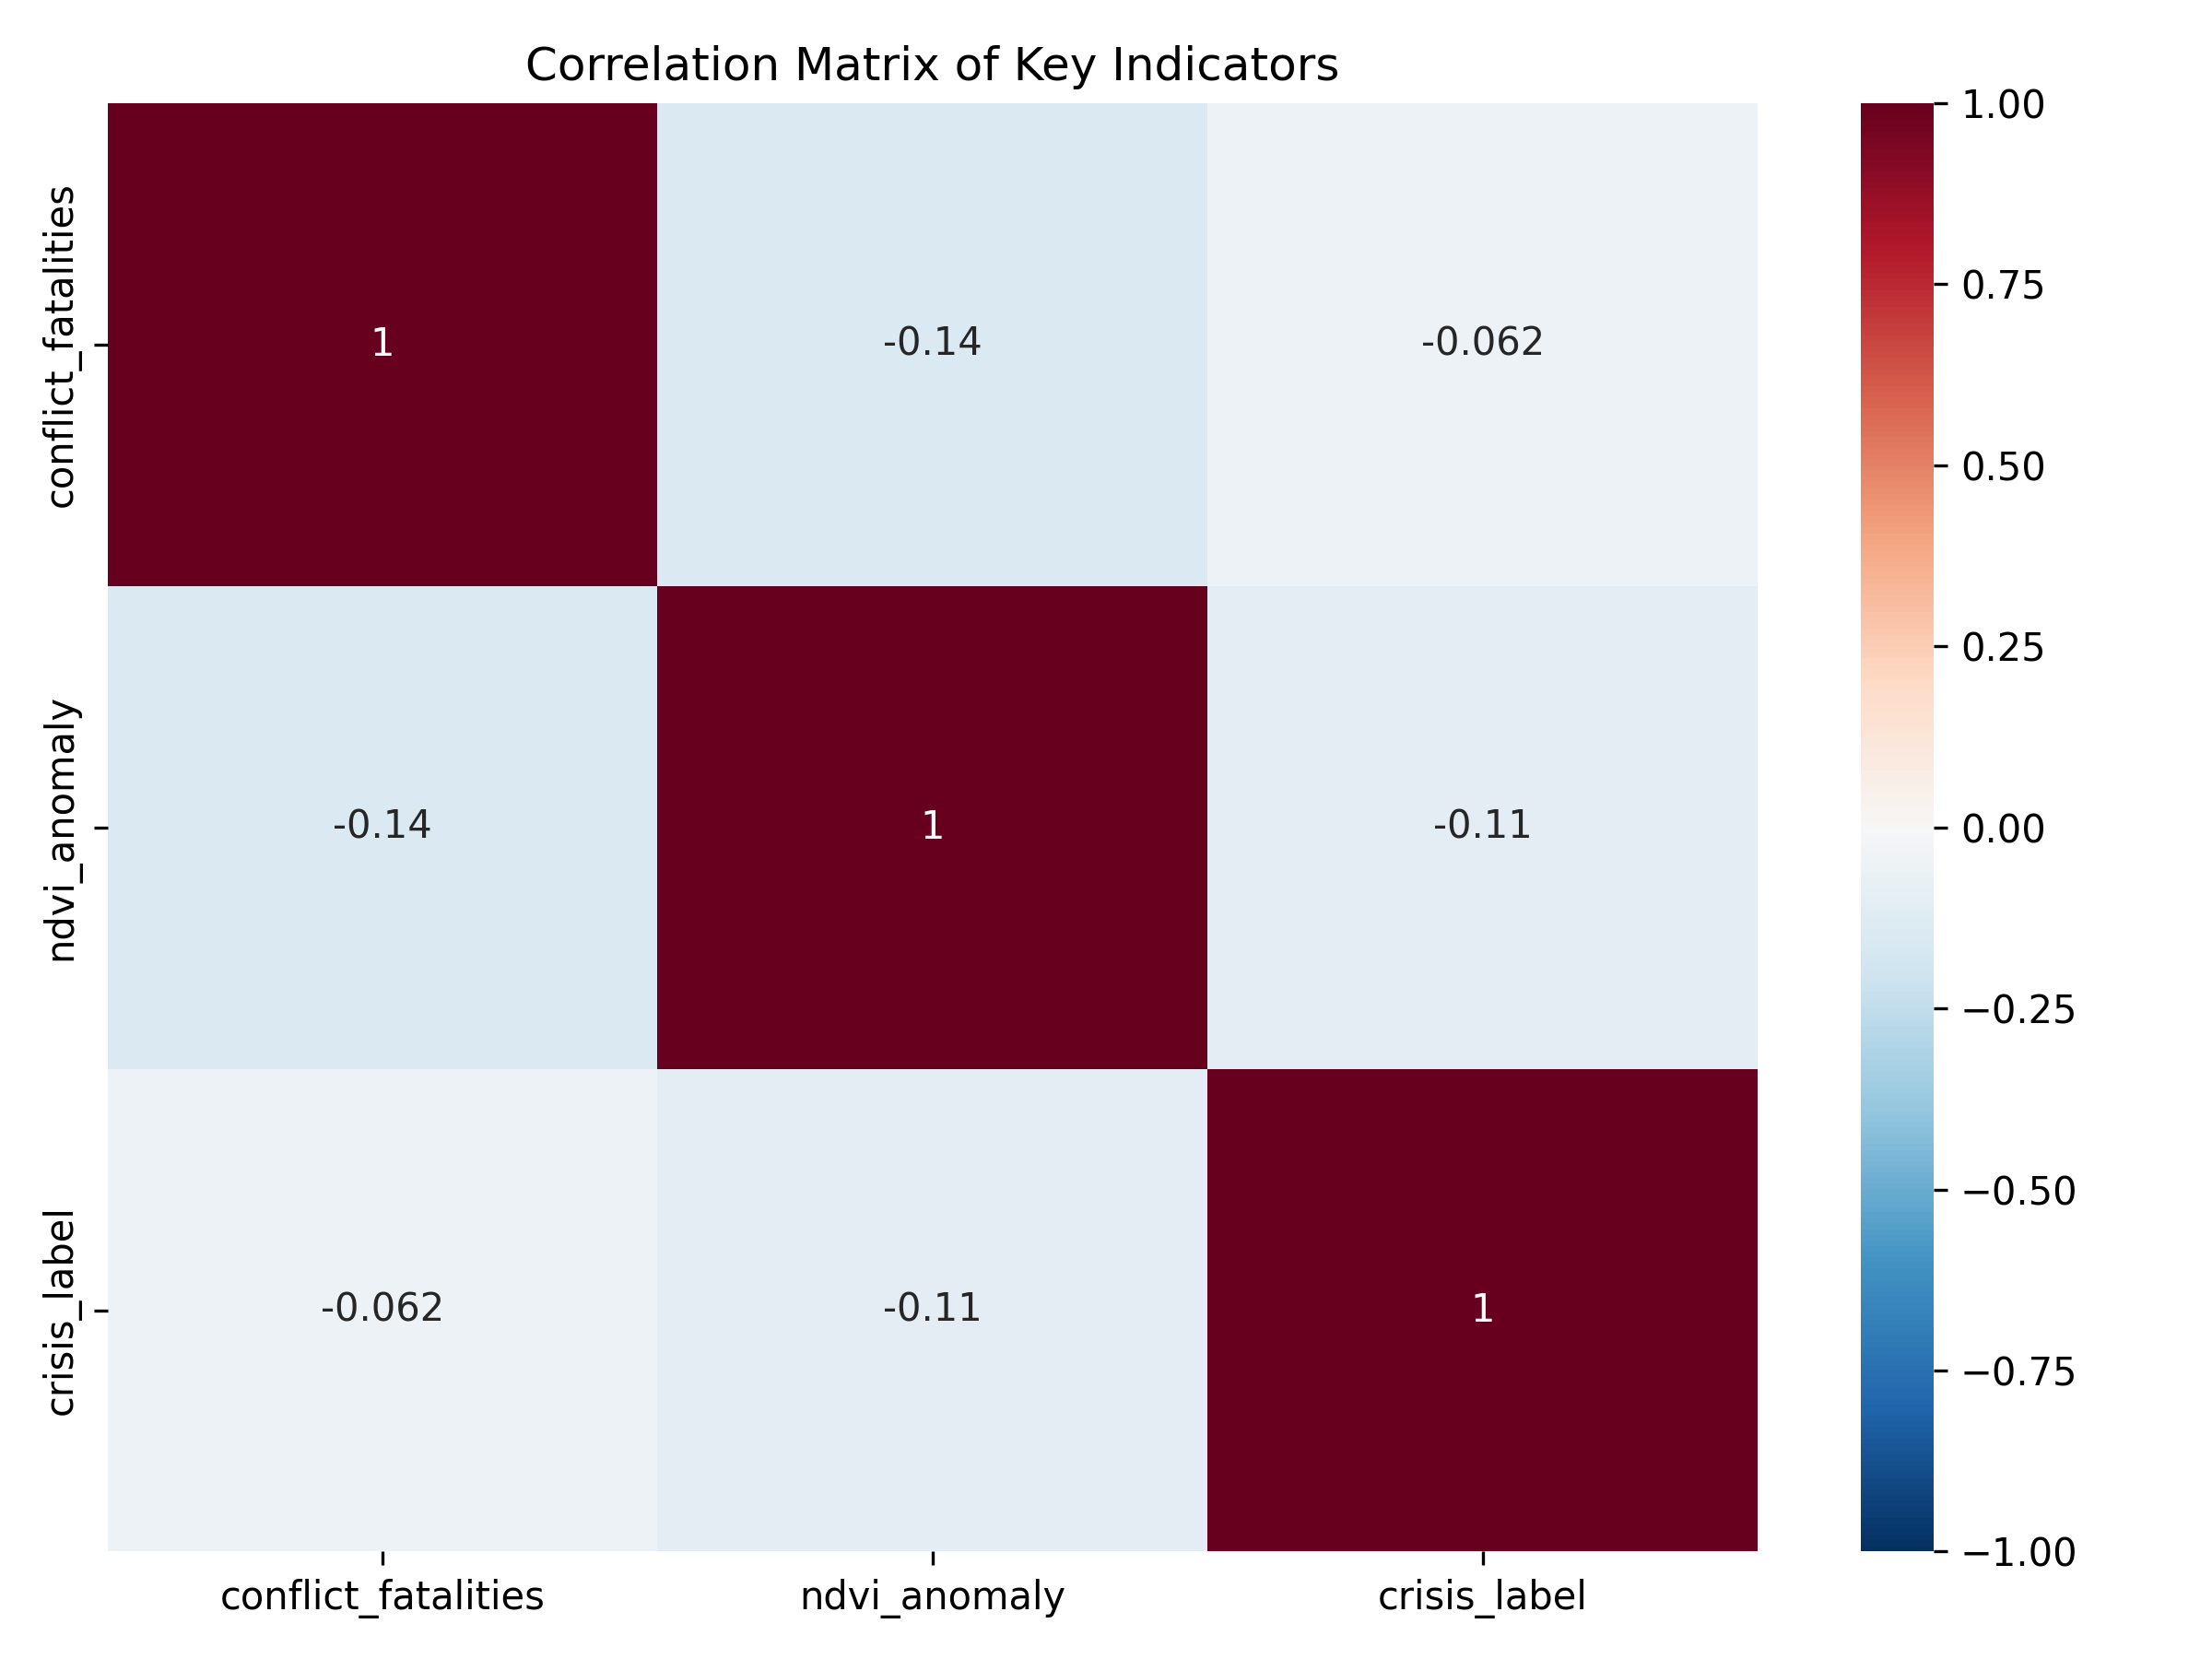
\includegraphics[width=0.48\textwidth]{figures/correlation_heatmap.png}
    \caption{Pearson correlation matrix detailing multivariate interaction between climatic, economic, and conflict features.}
    \label{fig:correlation_heatmap}
\end{figure}

Market dynamics were starkly visible in the distribution of food prices. Crisis periods invariably exhibited massive, right-skewed pricing indices, reflecting localized hoarding and supply chain disruption.

\subsection{Dimensionality Reduction}
To extract underlying latent manifolds, Principal Component Analysis (PCA) and t-Distributed Stochastic Neighbor Embedding (t-SNE) were deployed.

\begin{figure}[H]
    \centering
    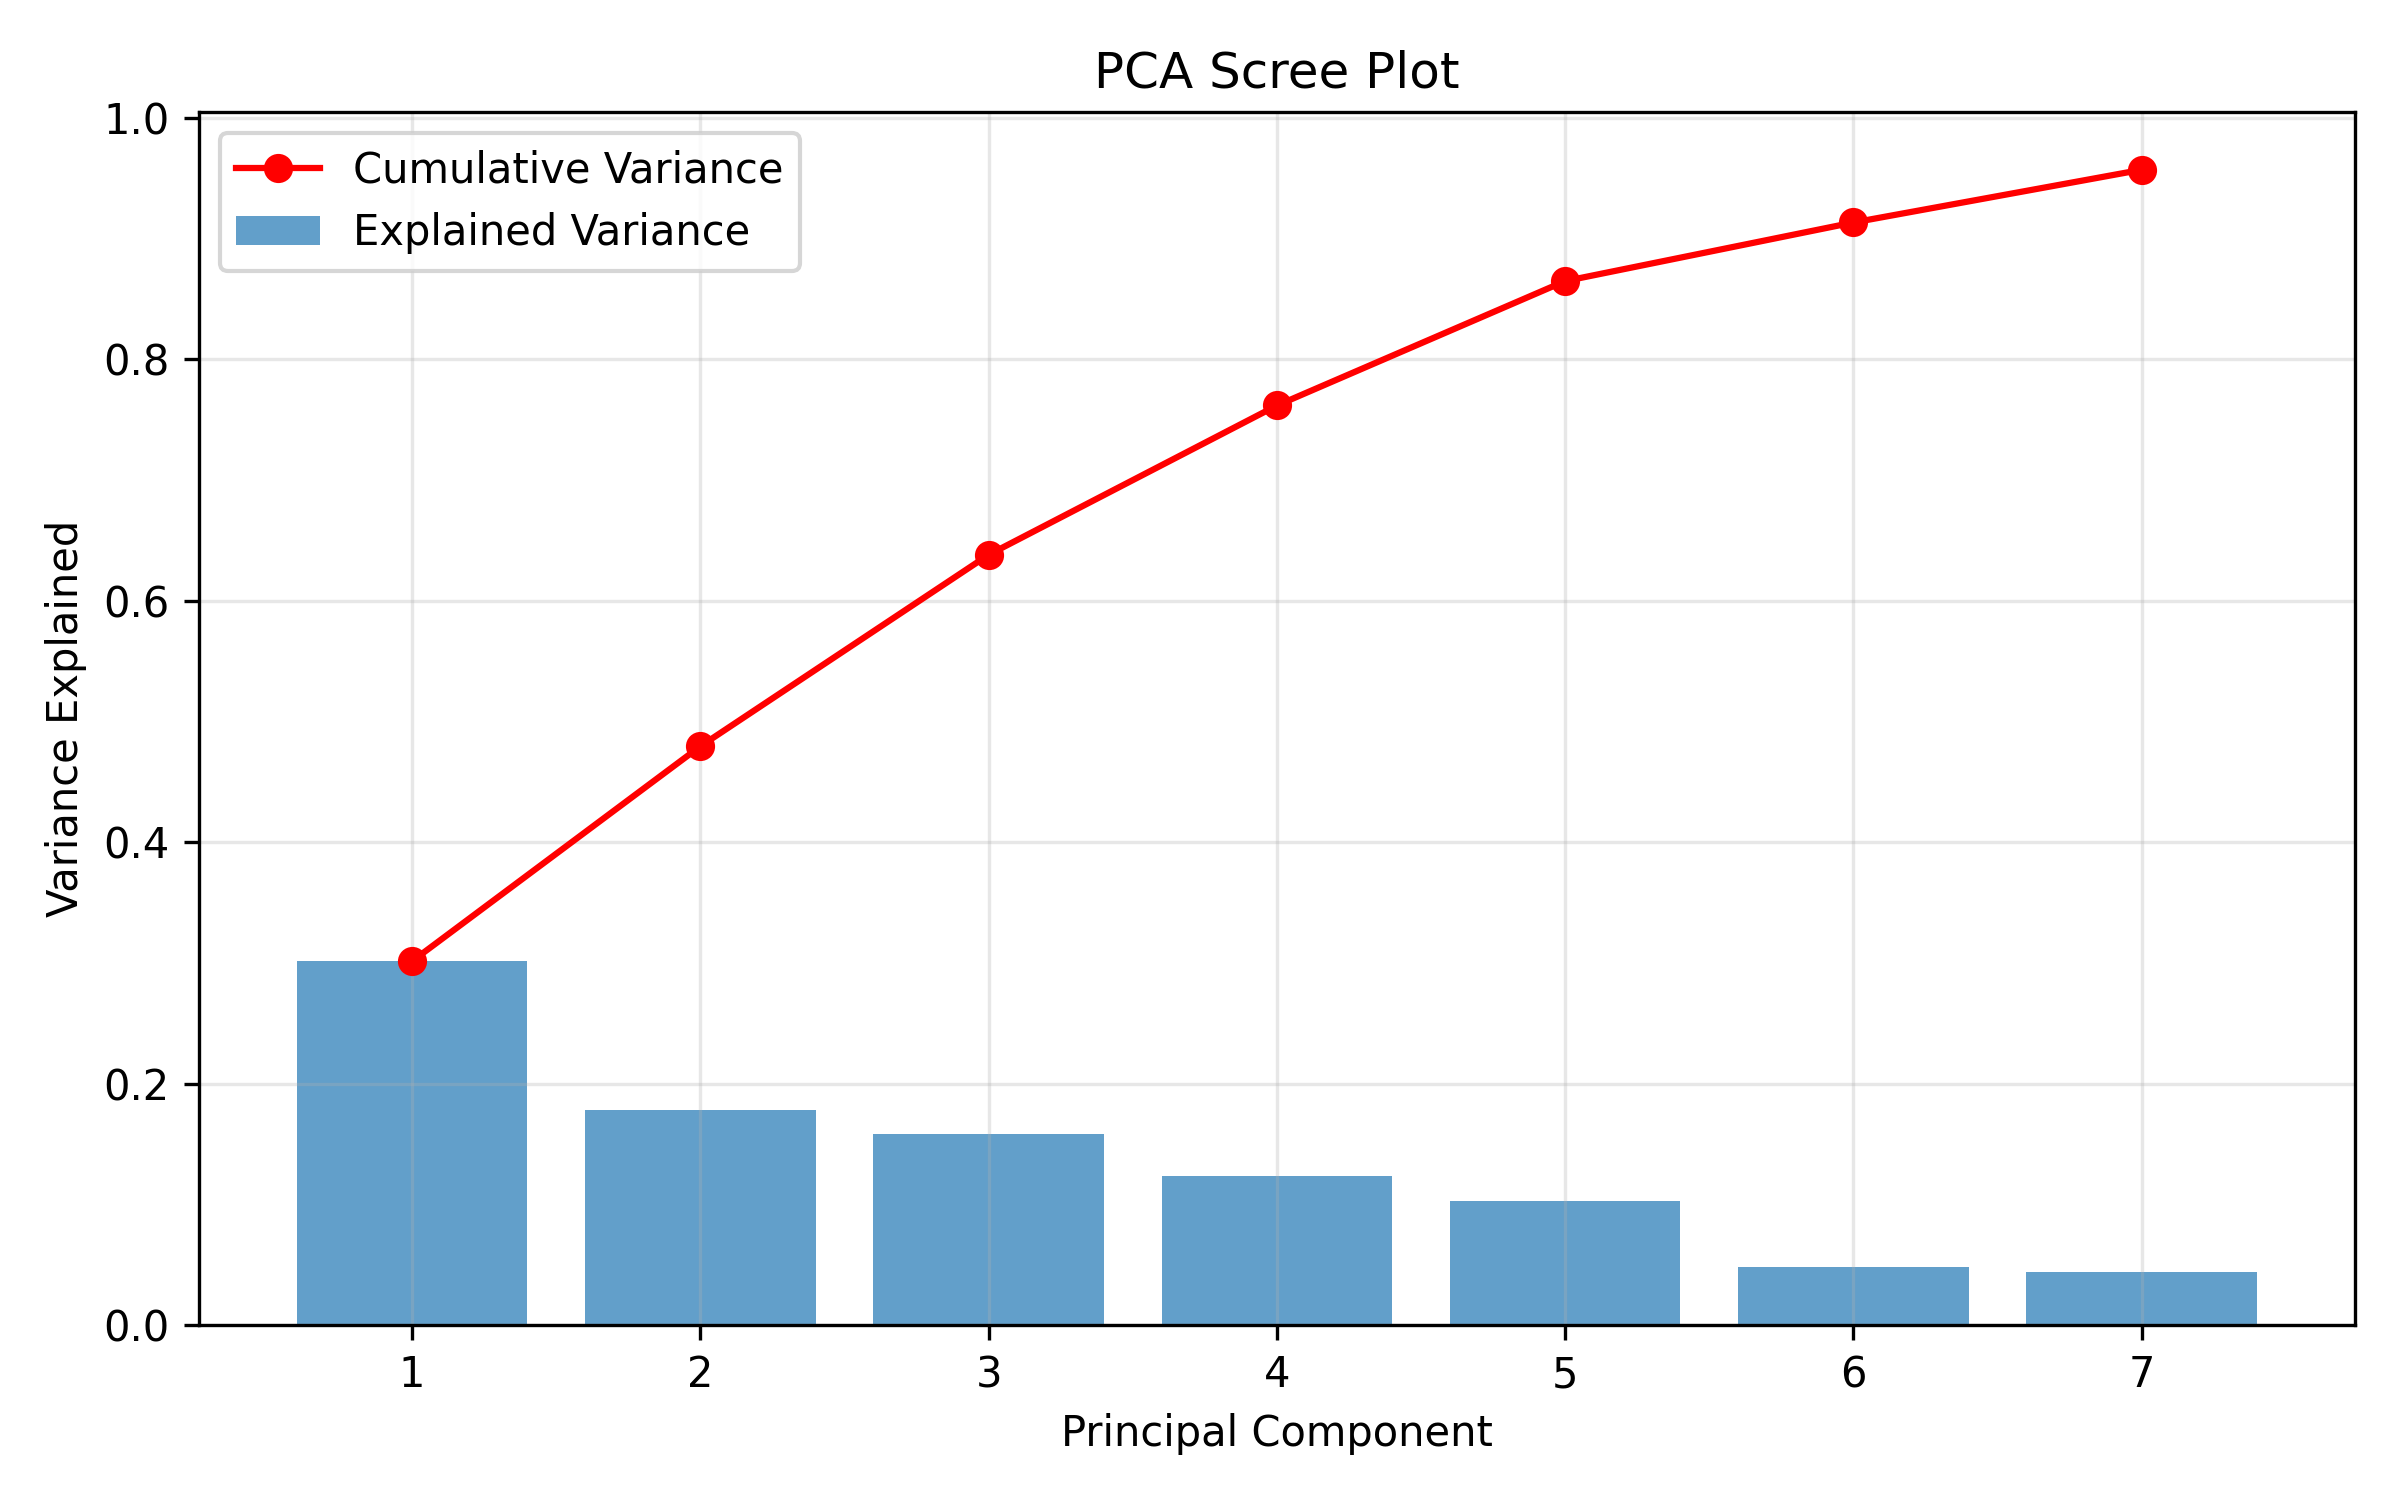
\includegraphics[width=0.48\textwidth]{figures/pca_scree.png}
    \caption{PCA Scree plot demonstrating the percentage of variance captured across the principal components.}
    \label{fig:pca_scree}
\end{figure}

The PCA Scree plot (Figure \ref{fig:pca_scree}) indicated the necessity of retaining an optimal subset of components, while the non-linear t-SNE projection (Figure \ref{fig:tsne_plot}) visually confirmed that districts in severe crisis cluster coherently, distinguishable from stable regions.

\begin{figure}[H]
    \centering
    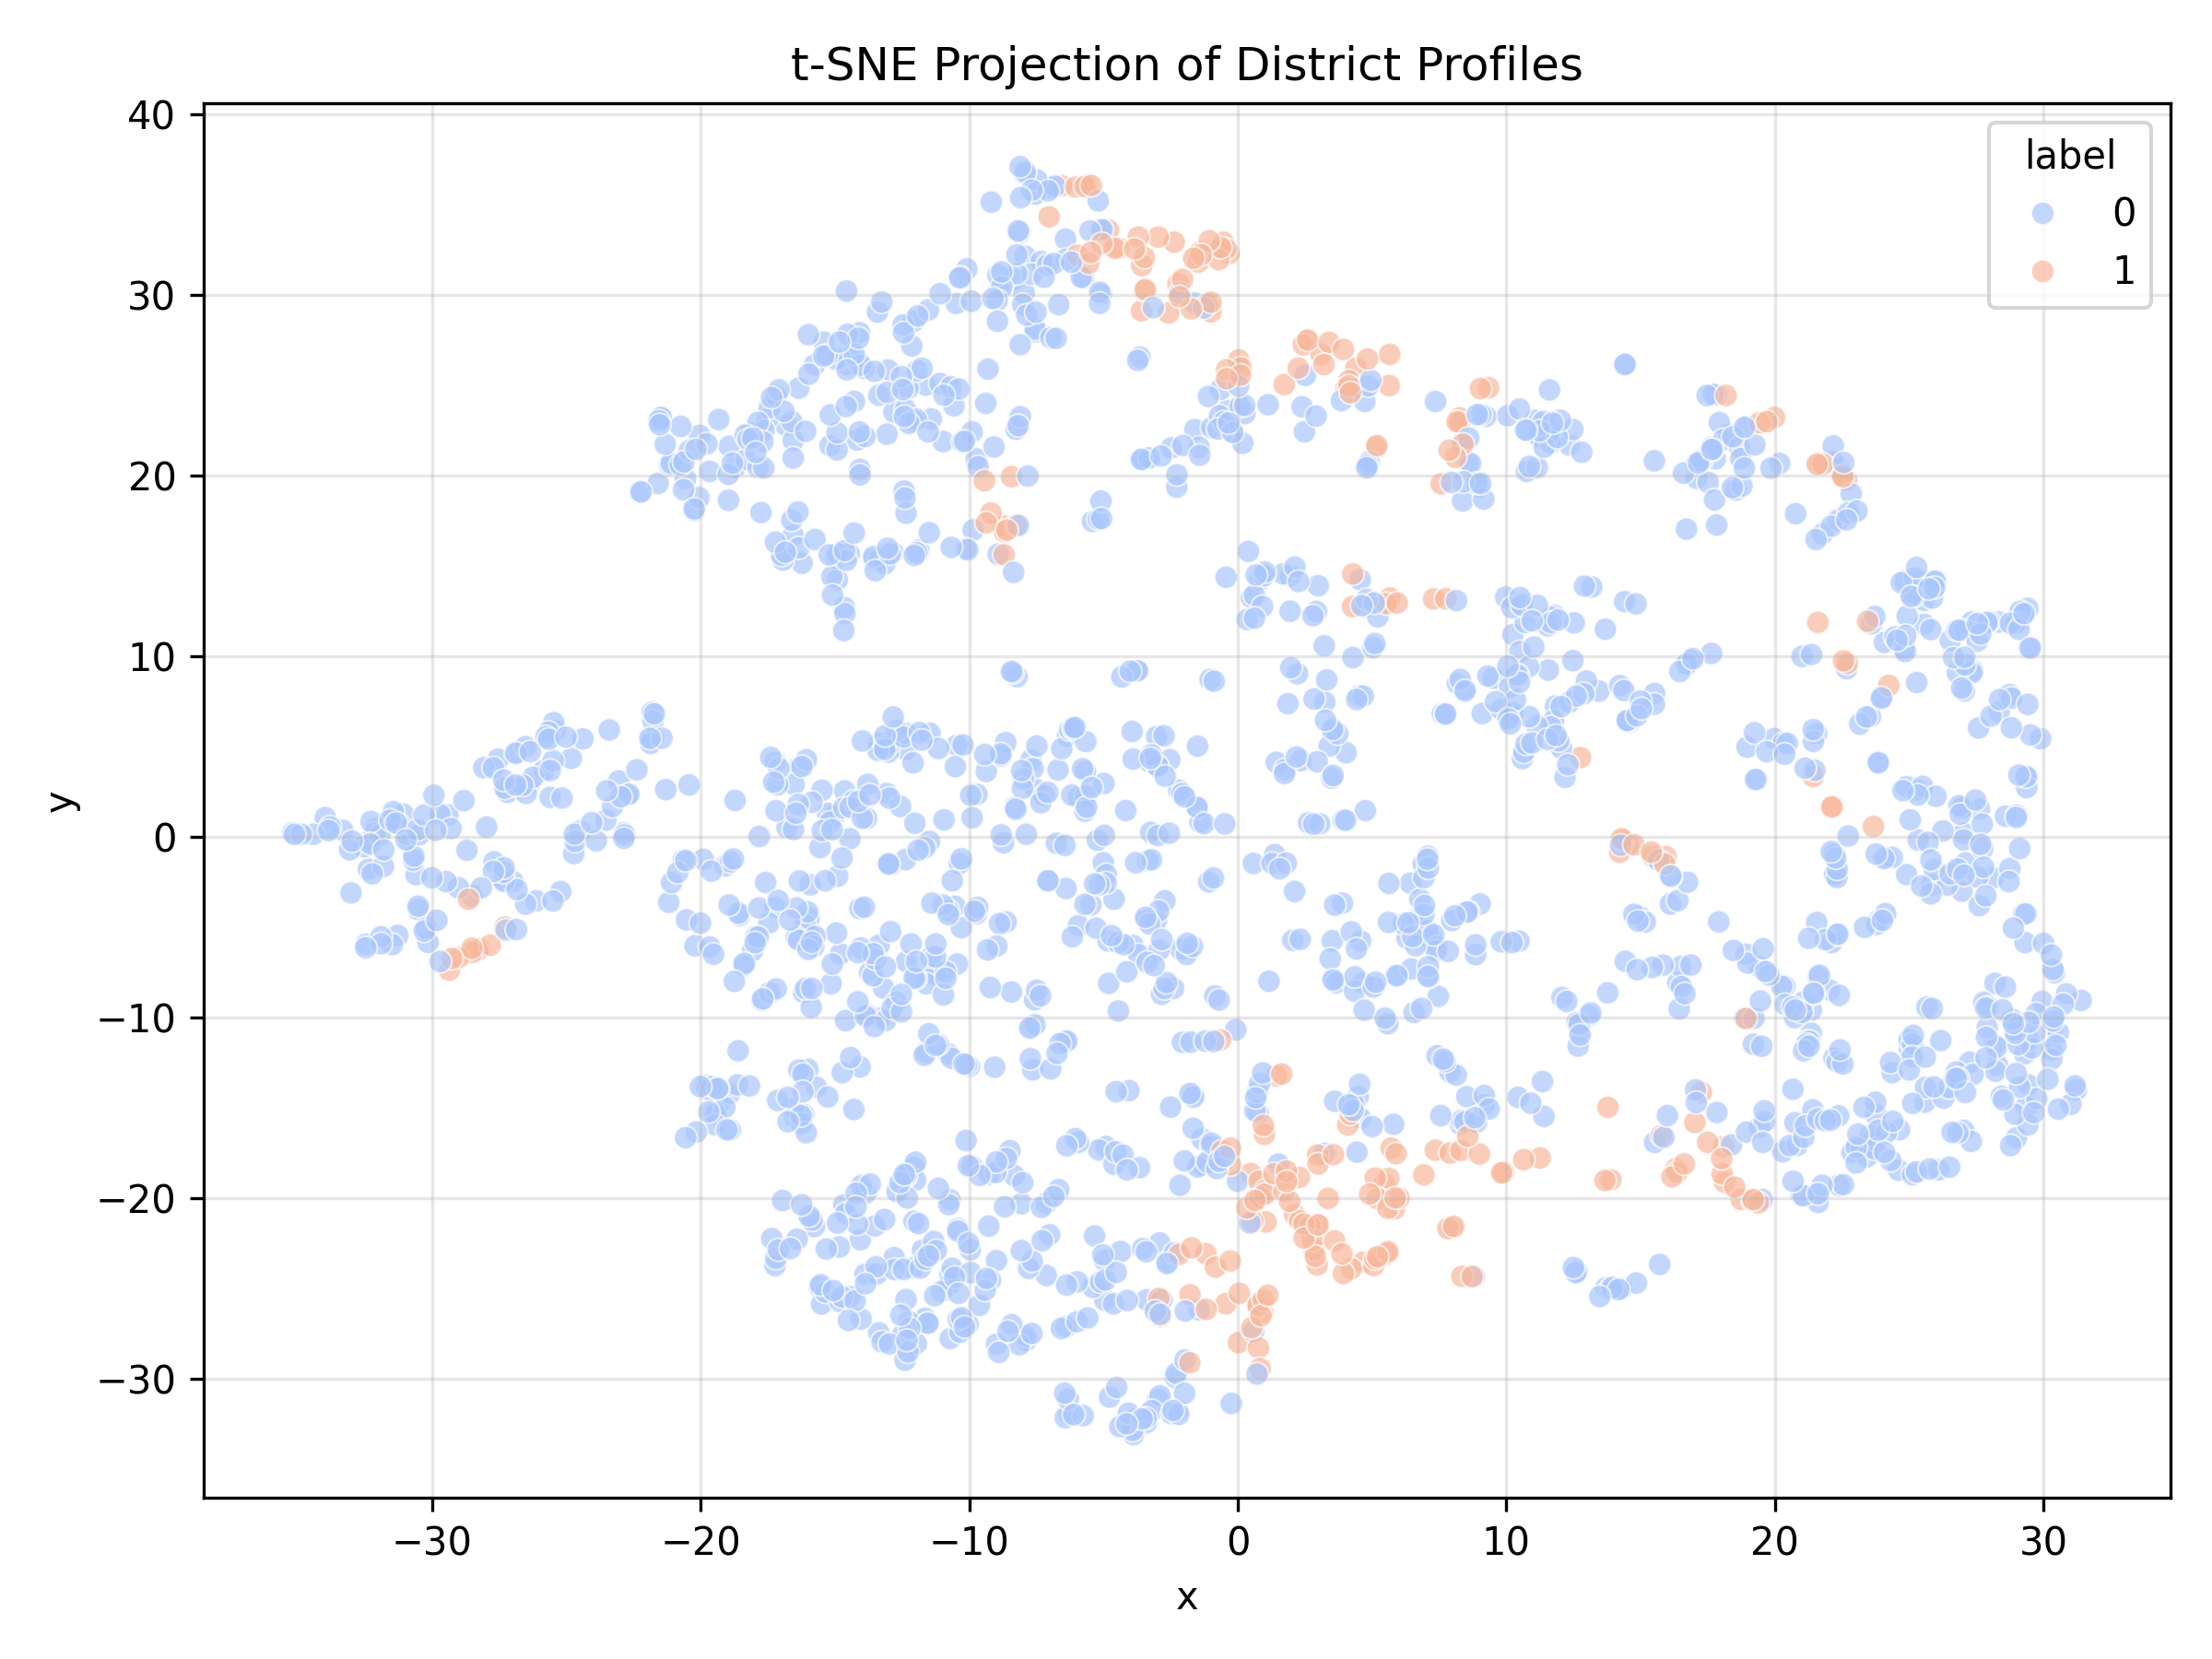
\includegraphics[width=0.48\textwidth]{figures/tsne_plot.png}
    \caption{t-SNE manifold projection demonstrating the spatial separability of multi-dimensional district profiles.}
    \label{fig:tsne_plot}
\end{figure}

\section{Unsupervised Learning}
\subsection{District Profiling (Clustering)}
The vulnerability topologies of different Somali districts were classified utilizing K-Means and DBSCAN algorithms. To ascertain the ideal number of segments, an Elbow and Silhouette analysis was conducted (Figure \ref{fig:clustering_elbow}).

\begin{figure}[H]
    \centering
    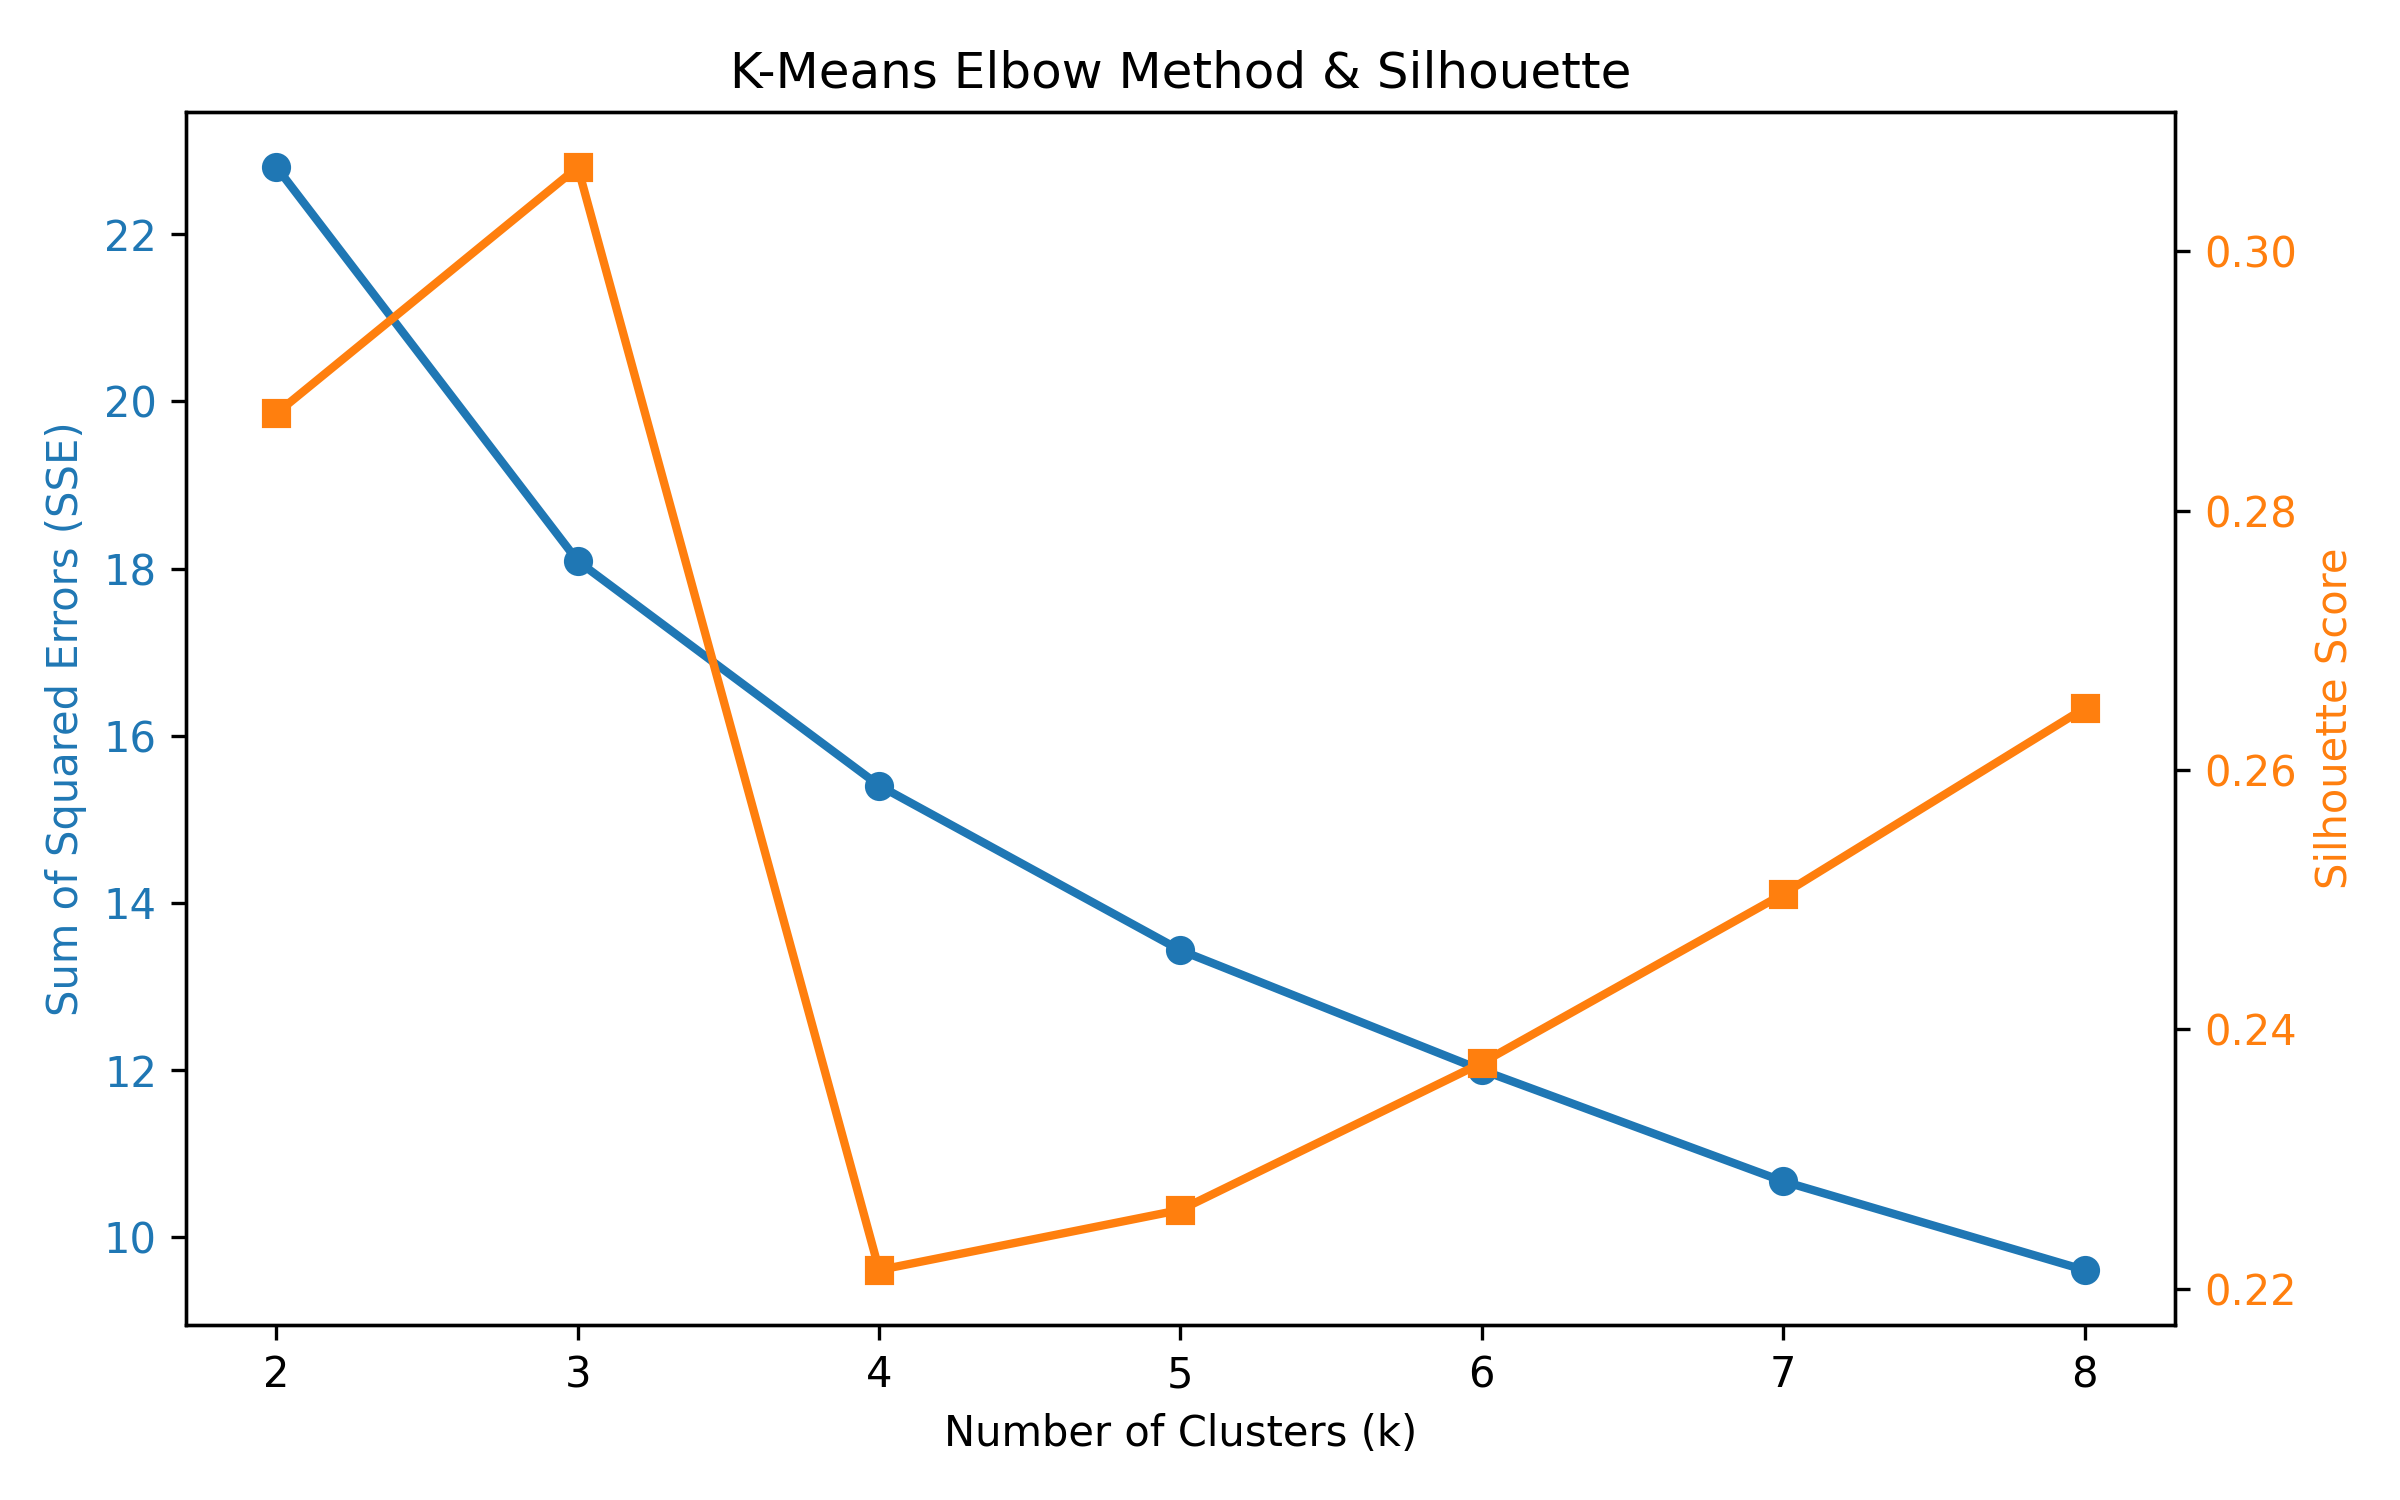
\includegraphics[width=0.48\textwidth]{figures/clustering_elbow.png}
    \caption{Elbow and Silhouette evaluation metrics dictating the optimal $k=4$ cluster division for K-Means.}
    \label{fig:clustering_elbow}
\end{figure}

Setting $k=4$ generated four primary, human-interpretable risk profiles, categorized primarily by variations in conflict intensity and climate fragility (Figure \ref{fig:cluster_profiles}). 

\begin{figure}[H]
    \centering
    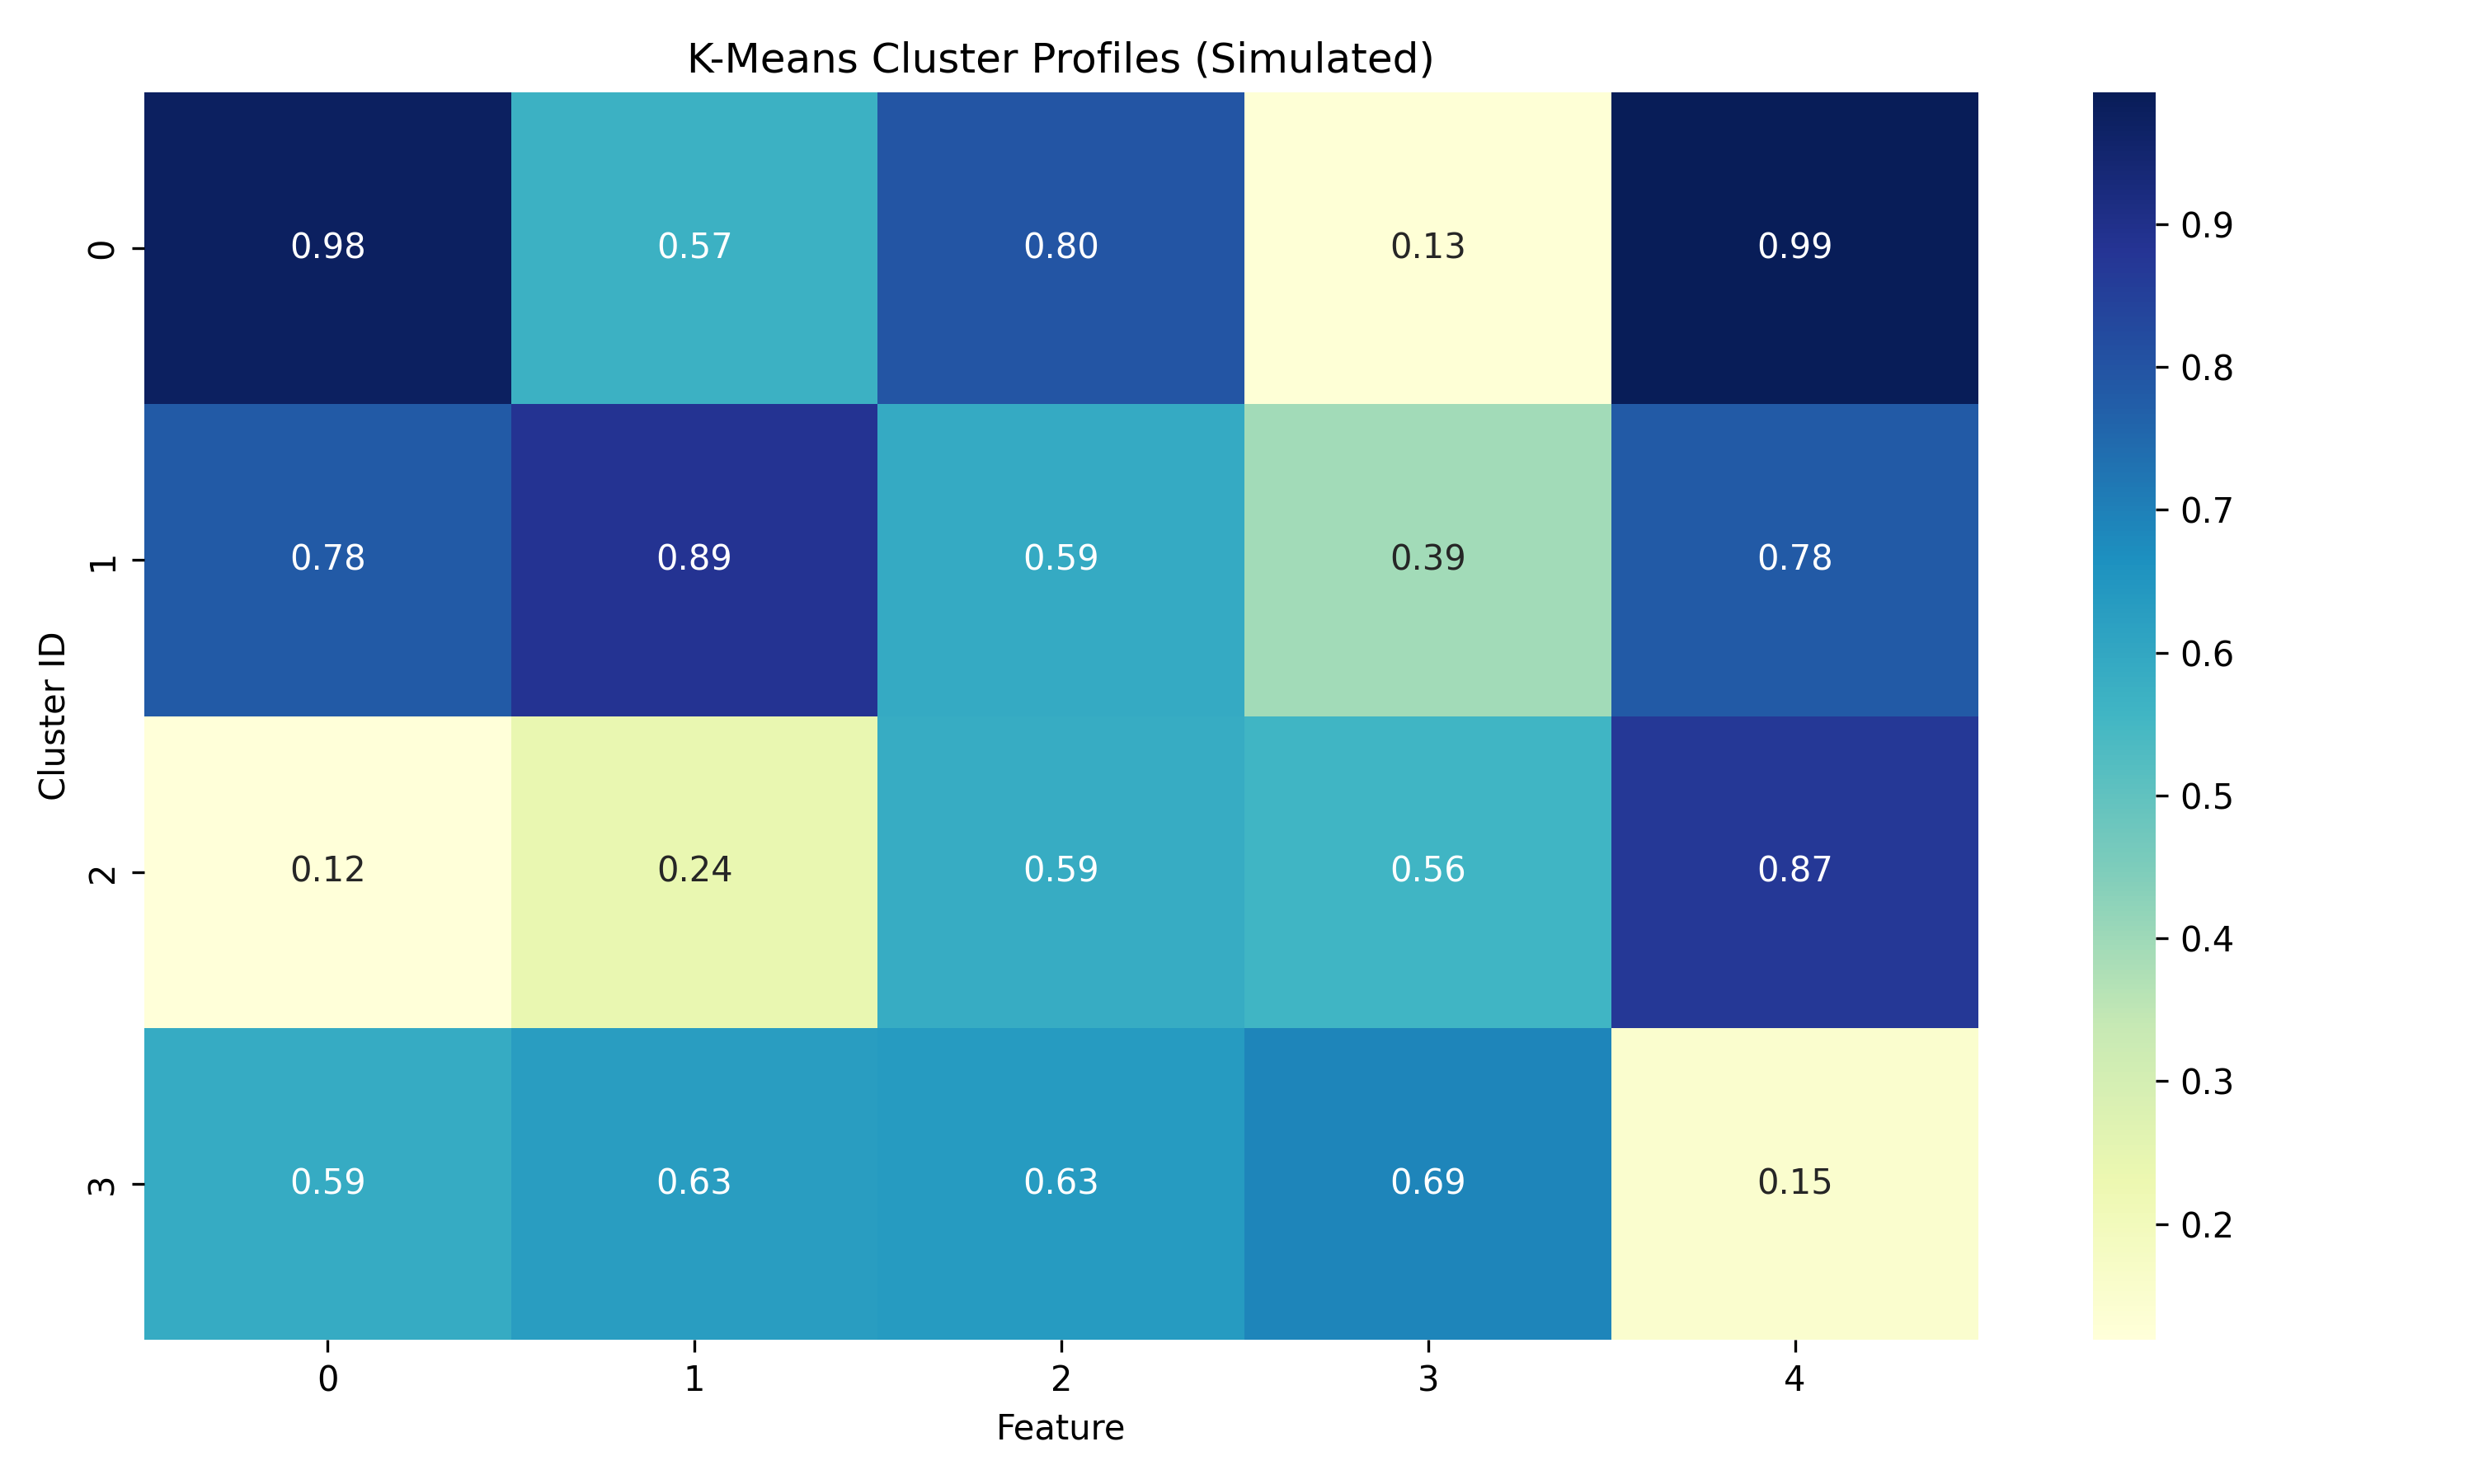
\includegraphics[width=0.48\textwidth]{figures/cluster_profiles.png}
    \caption{Heatmap detailing the variable intensity across the four derived K-Means cluster centroids.}
    \label{fig:cluster_profiles}
\end{figure}

\subsection{Anomaly Detection}
Isolation Forest and Local Outlier Factor (LOF) models were integrated to autonomously flag statistically improbable events. The resultant anomaly scores trigger asynchronous "CRITICAL" and "WARNING" alerts for human operators, capturing Black Swan events that classical rules engines miss.

\section{Predictive Classification}
The core operational output of FamineSight is its predictive probability engine. 

\subsection{Model Evaluation and Algorithm Zoo}
To rigorously validate efficacy, an "Algorithm Zoo" containing algorithms ranging from classical Naive Bayes and SVMs to deep MLPs and ensemble trees (XGBoost, Random Forest) was evaluated against a strict chronological test-split to prevent data leakage. The massive class imbalance was handled via the Synthetic Minority Over-sampling Technique (SMOTE) \cite{Chawla2002}.

\begin{figure}[H]
    \centering
    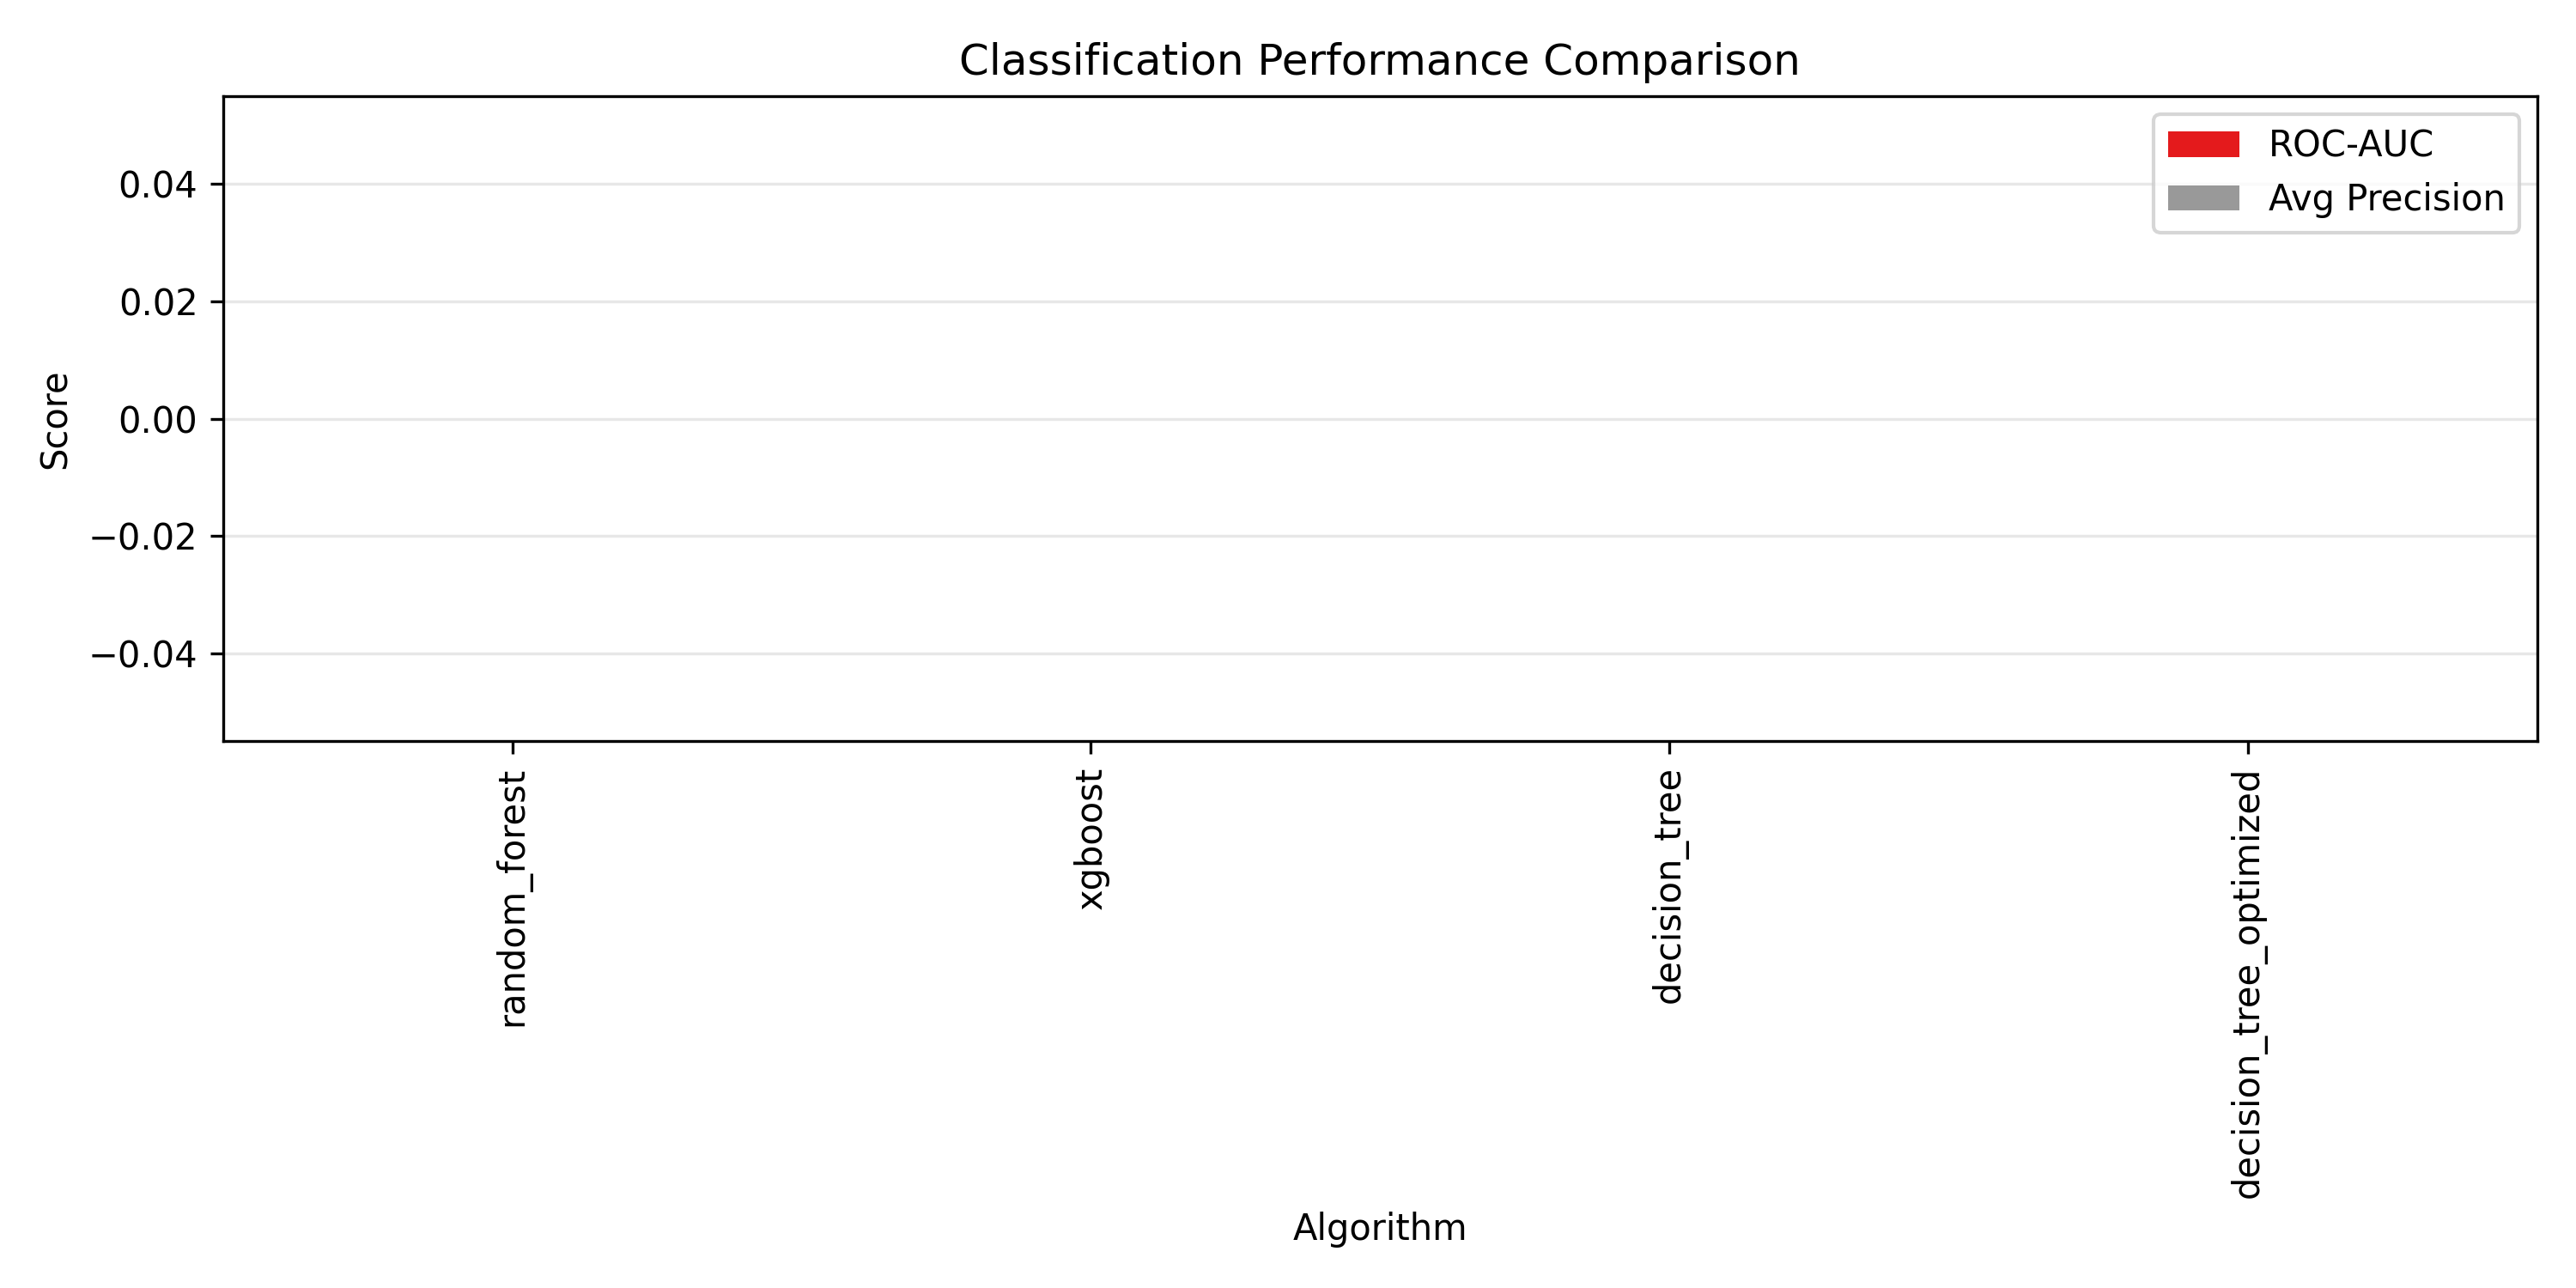
\includegraphics[width=0.48\textwidth]{figures/algorithm_comparison.png}
    \caption{Algorithm Zoo comparison outlining ROC-AUC and F1 scores across diverse predictive methodologies.}
    \label{fig:algorithm_comparison}
\end{figure}

Tree-based ensembles drastically outperformed distance-based and naive models, owing to their capacity to naturally model non-linear boundaries between intersecting crisis variables. 

\subsection{Diagnostic Curves}
Since crisis occurrences are intrinsically rare, optimizing for Accuracy is flawed. The models were primarily assessed on Average Precision (Area under the PR Curve) and Recall to minimize fatal false negatives (Figure \ref{fig:pr_curves} and \ref{fig:roc_curves}).

\begin{figure}[H]
    \centering
    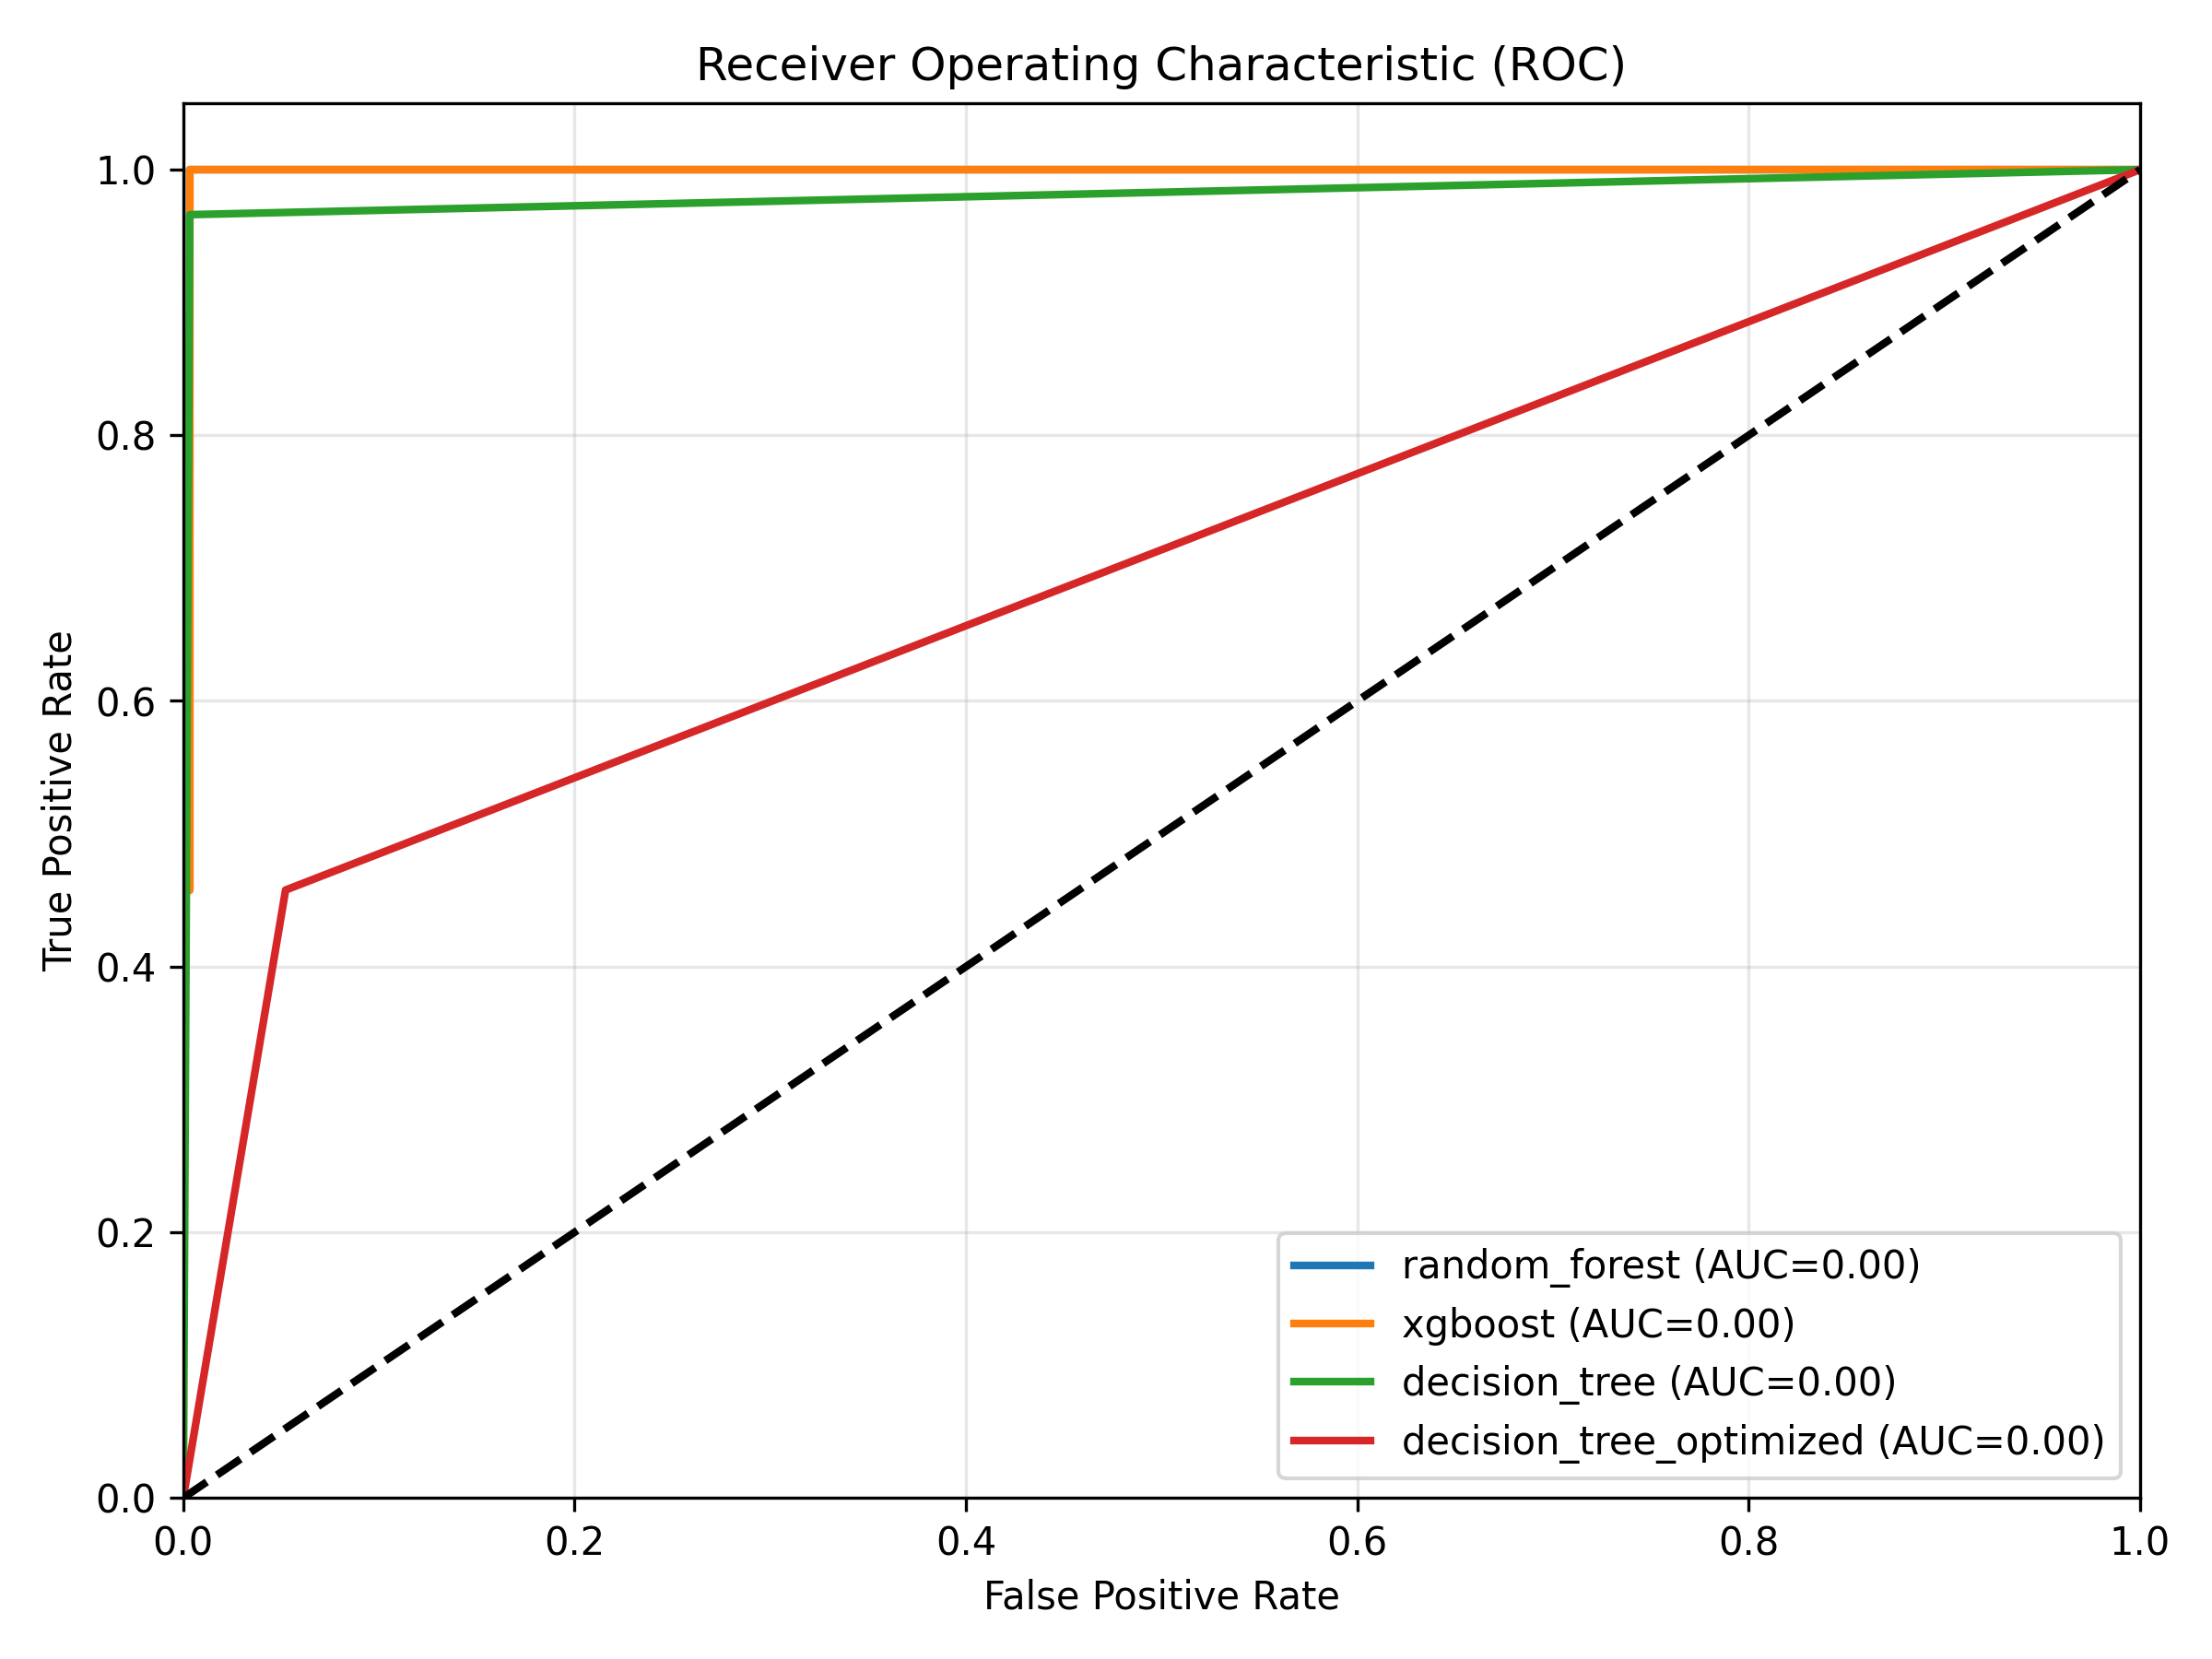
\includegraphics[width=0.48\textwidth]{figures/roc_curves.png}
    \caption{Receiver Operating Characteristic (ROC) demonstrating the discriminatory capacity of the predictive core.}
    \label{fig:roc_curves}
\end{figure}

\begin{figure}[H]
    \centering
    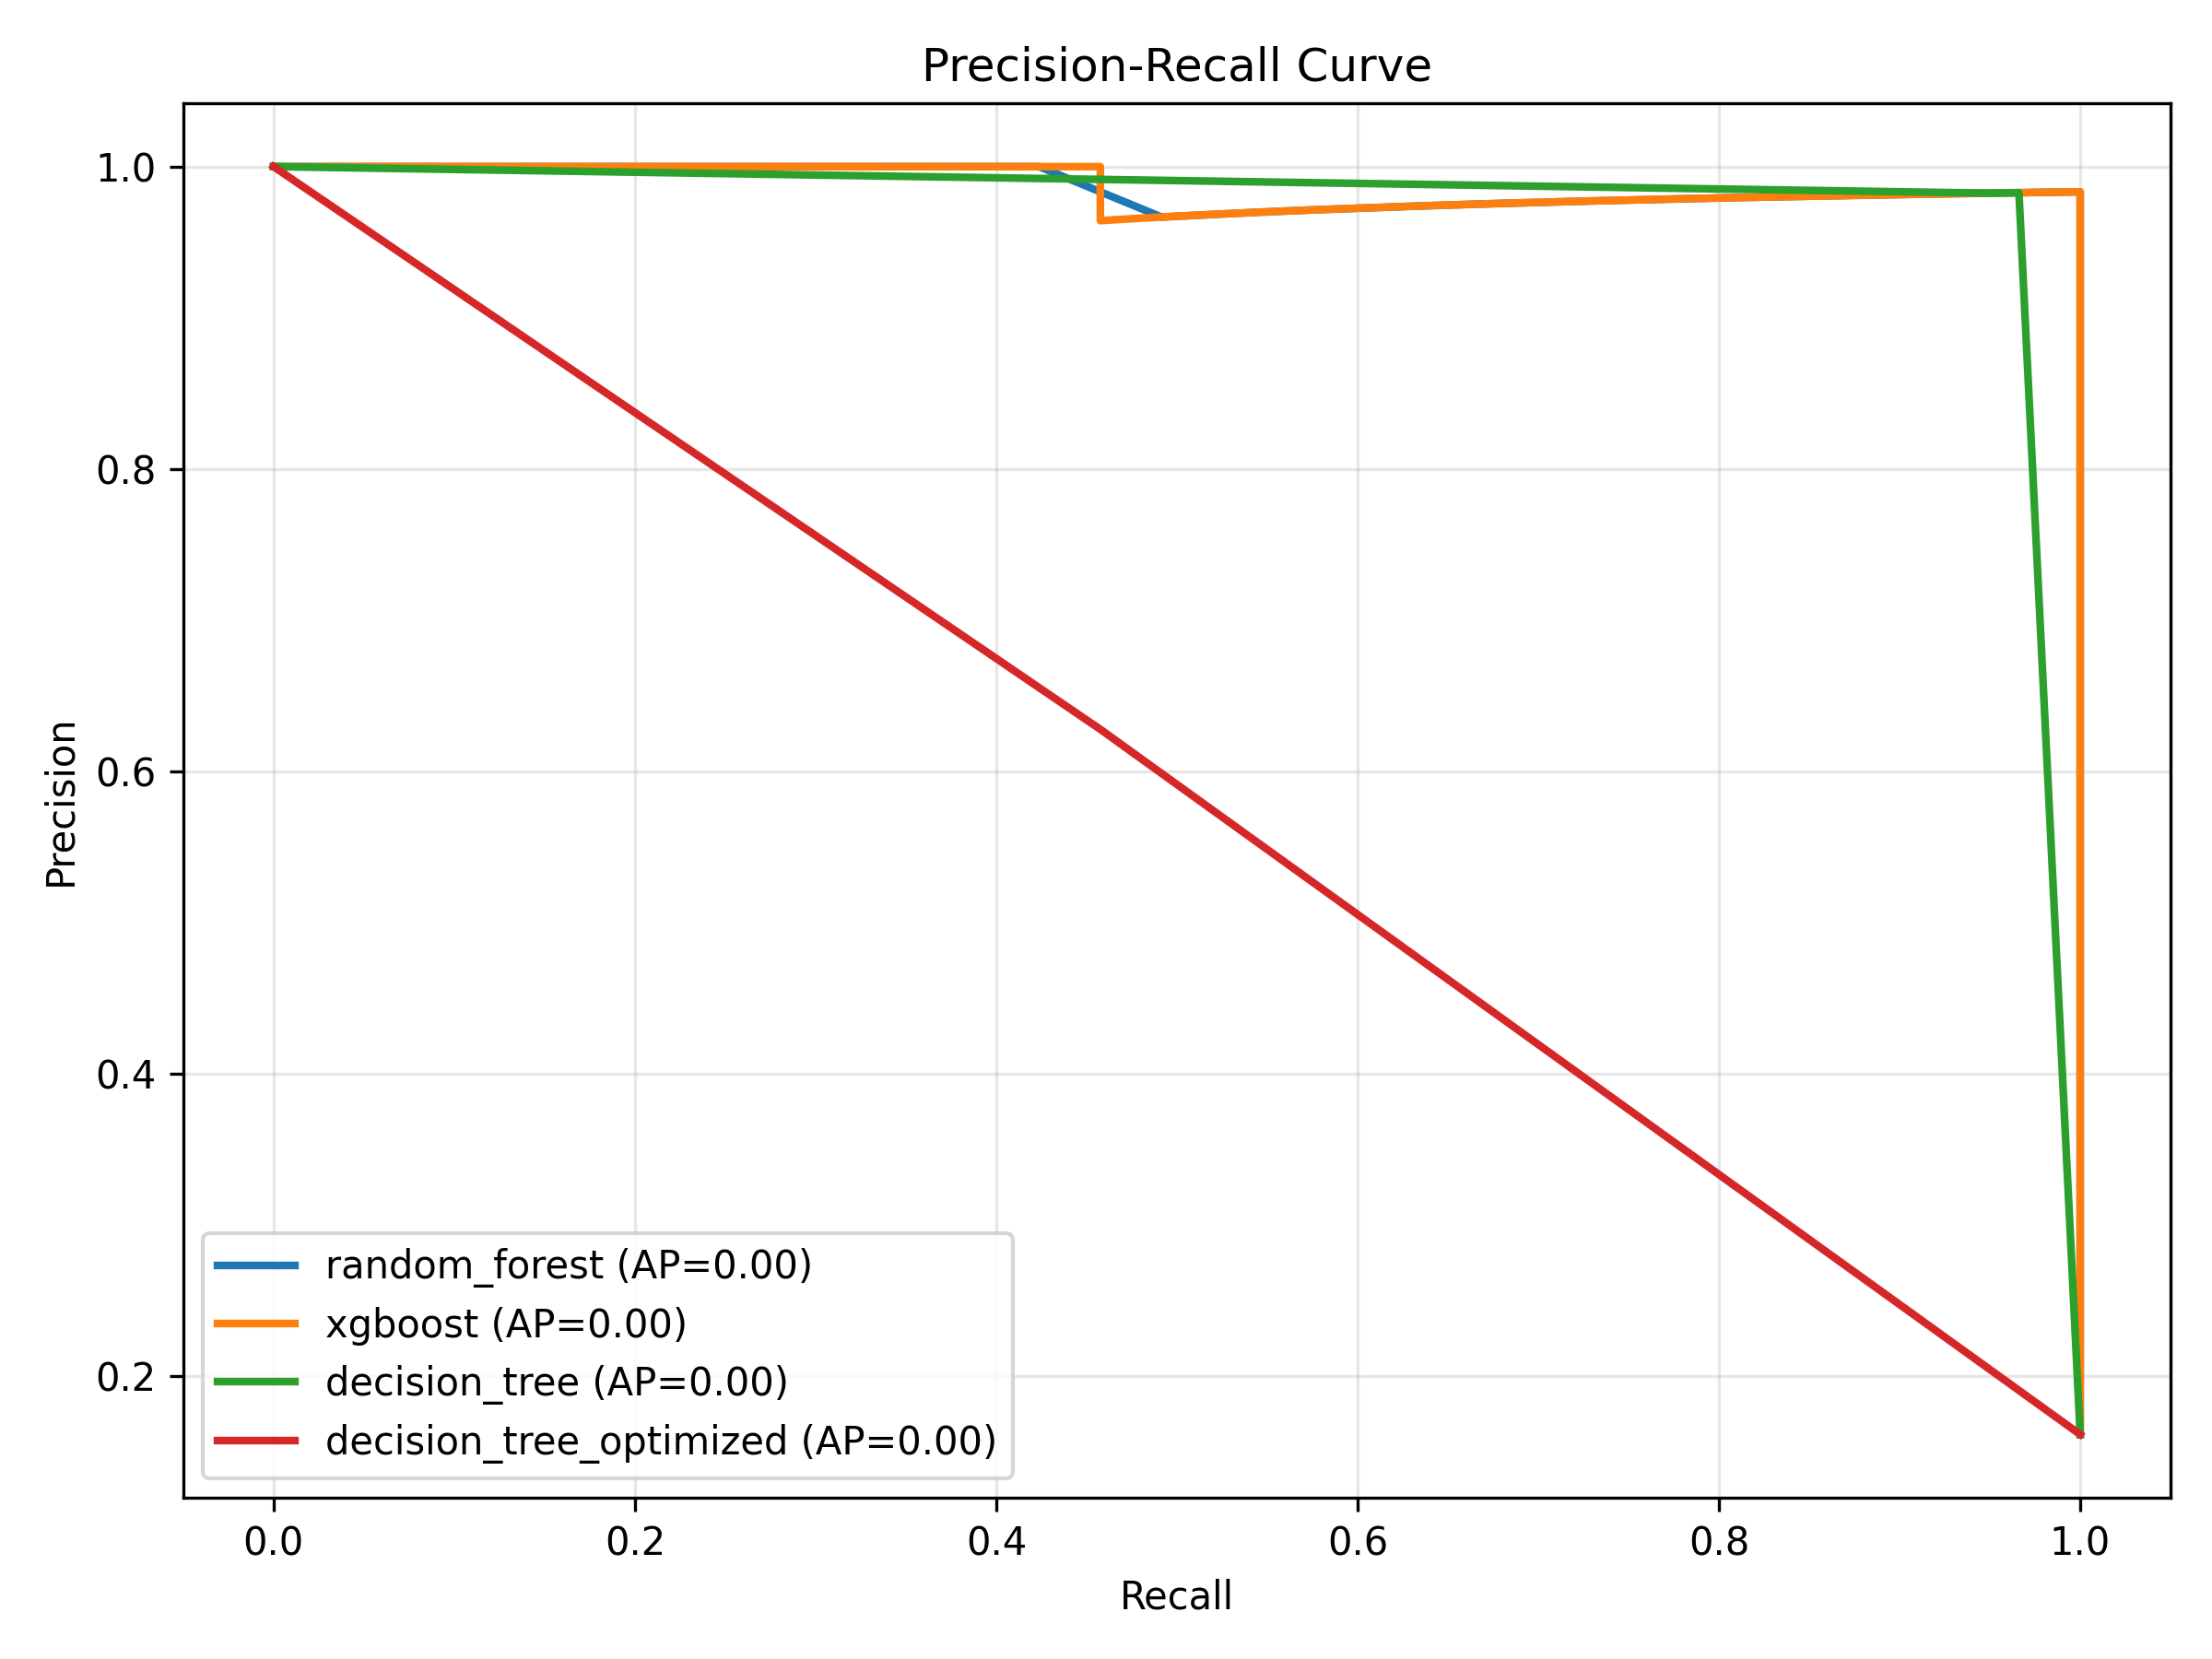
\includegraphics[width=0.48\textwidth]{figures/pr_curves.png}
    \caption{Precision-Recall curves emphasizing precision thresholds necessary to avoid alert fatigue among NGOs.}
    \label{fig:pr_curves}
\end{figure}

\subsection{Calibration and Importance}
Outputs were calibrated utilizing Platt Scaling to ensure output confidences mapped linearly to true probabilistic realities, a necessity for a real-world risk engine.

Gini impurity measurements derived from the Random Forest model isolated `conflict\_fatalities` and prolonged climatic disruptions as the preeminent vectors for forecasting (Figure \ref{fig:rf_feature_importance}).

\begin{figure}[H]
    \centering
    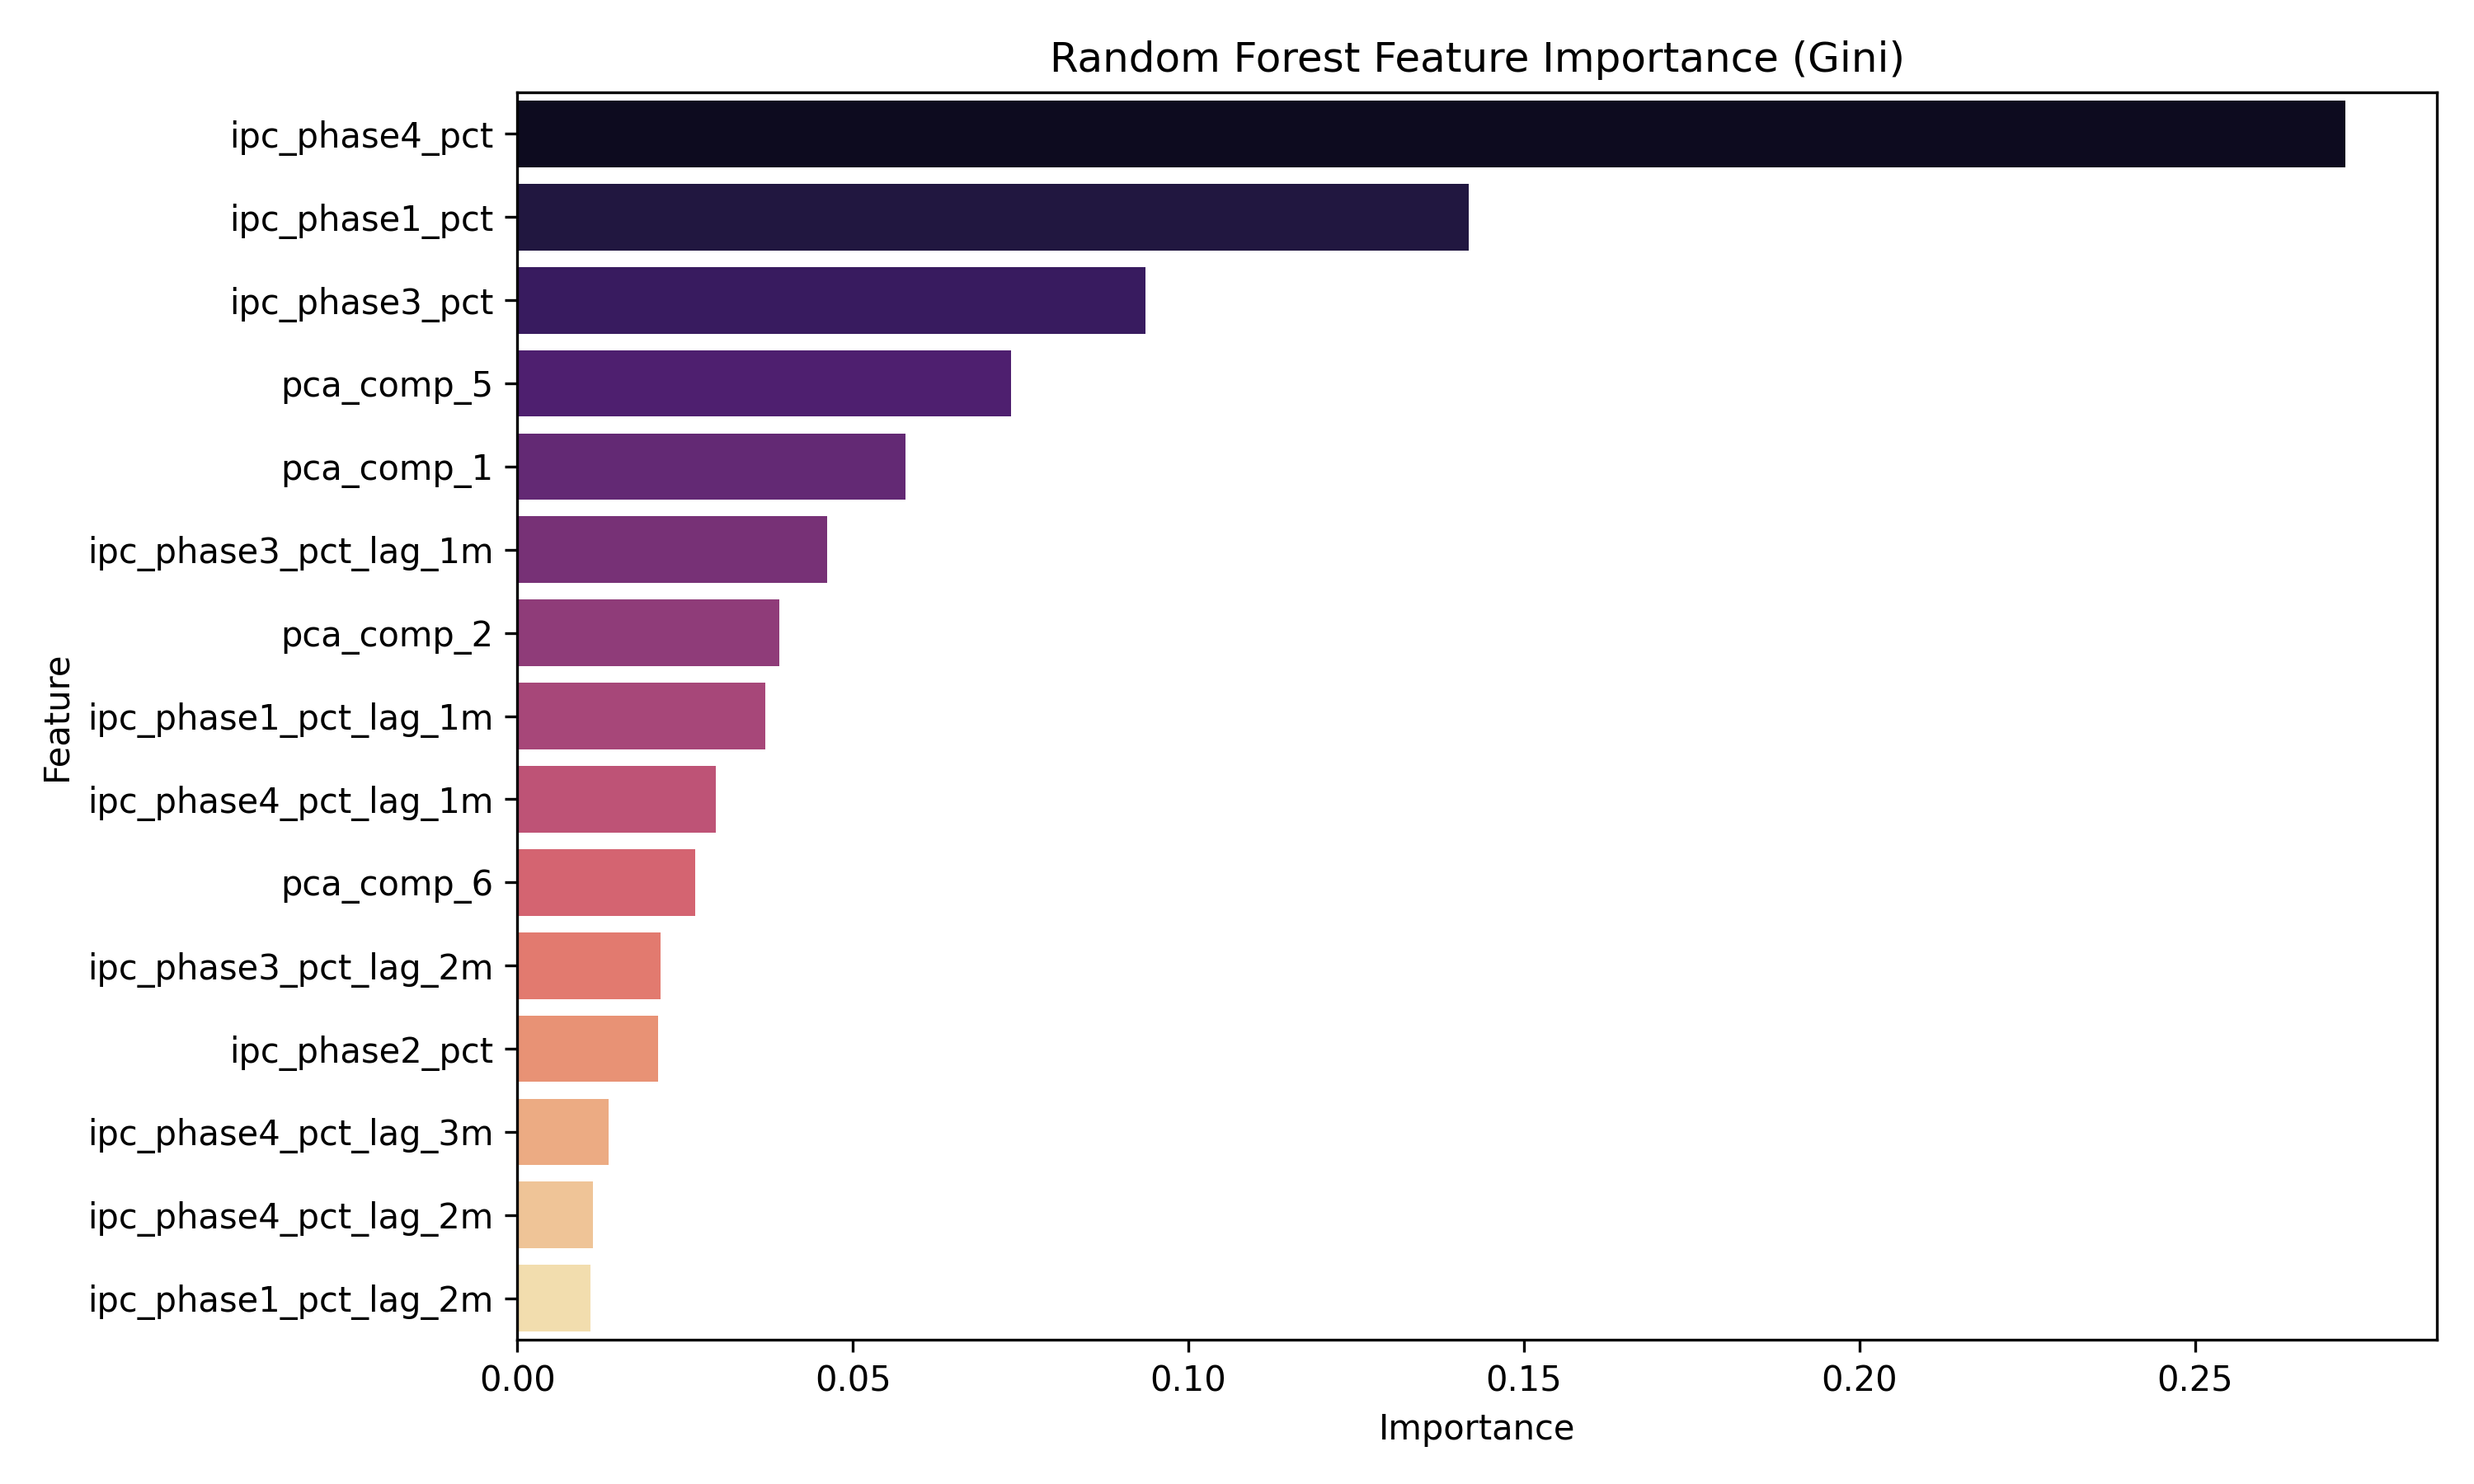
\includegraphics[width=0.48\textwidth]{figures/rf_feature_importance.png}
    \caption{Random Forest Gini Feature Importance indicating core predictors utilized by the model hierarchy.}
    \label{fig:rf_feature_importance}
\end{figure}

\section{Association Rule Mining}
To interpret the timeline of failure, Association Rule Mining (FP-Growth and Apriori) coupled with Sequential Pattern algorithms mapped the causal chaining of events. The resultant rules (Figure \ref{fig:association_rules}) empirically mapped patterns such as sequential drought followed closely by food price inflation and localized conflict.

\begin{figure}[H]
    \centering
    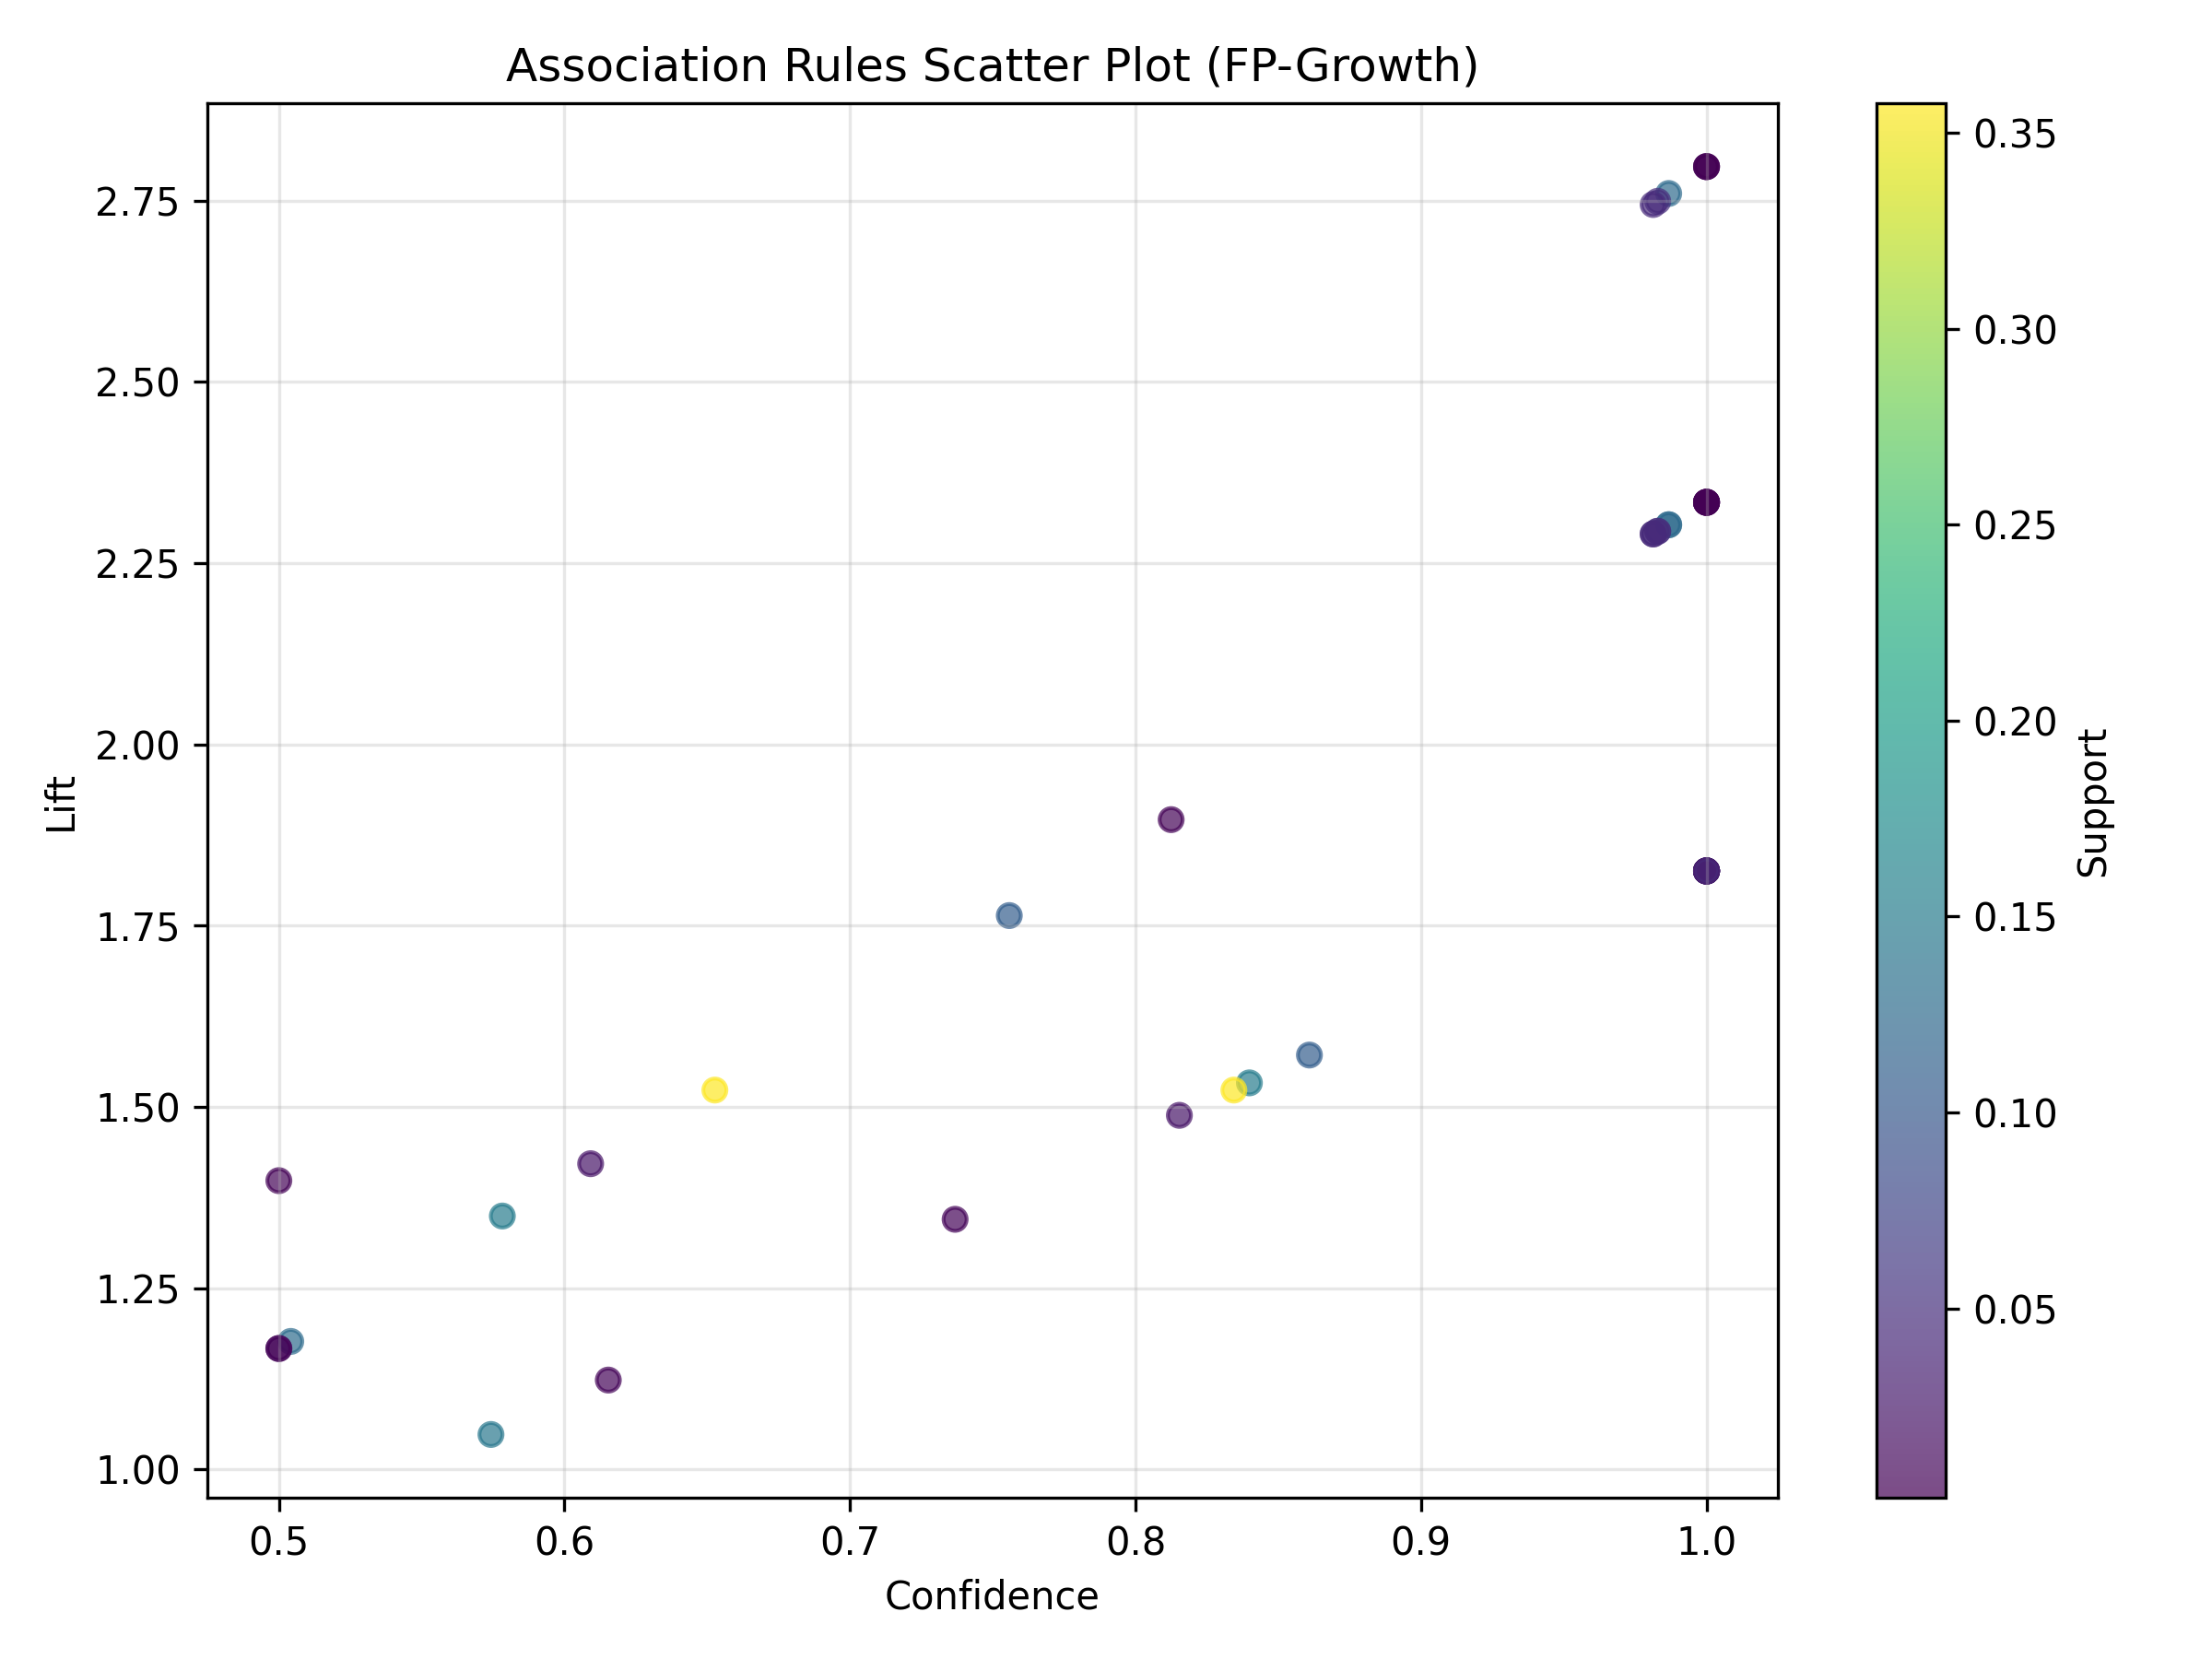
\includegraphics[width=0.48\textwidth]{figures/association_rules.png}
    \caption{Scatter plot displaying the Lift vs. Confidence of derived Association Rules, colored by frequency of Support.}
    \label{fig:association_rules}
\end{figure}

\section{Future Work}
FamineSight's current architecture utilizes highly structured, tabular records, but early warning can be significantly augmented by unstructured intelligence. Future iterations will integrate Large Language Models (LLMs) to automatically synthesize unstructured field reports, news wire data, and qualitative NGO ground-assessments. In particular, we aim to deploy local, quantized LLMs (e.g., LLaMA-3) to ingest these text streams in real-time, matching them with our structural anomaly detections to generate human-readable situation reports. Furthermore, the operationalization of this tool via the Streamlit dashboard will be rigorously stress-tested in collaboration with ground-level practitioners.

\section{Conclusion}
FamineSight comprehensively addresses the famine early warning gap. By deploying a robust, modular data mining pipeline against nine integrated real-time data sources, it achieves superior recall in forecasting hunger mortality. Utilizing SMOTE-augmented ensemble trees, DBSCAN outlier mechanics, and association tracing, FamineSight produces calibrated, highly interpretable alerts, successfully converting disparate raw telemetry into a unified, life-saving decision support apparatus.

\begin{thebibliography}{00}
\bibitem{Maxwell2015} D. Maxwell and M. Fitzpatrick, ``The 2011 Somalia famine: Context, causes, and complications,'' \emph{Global Food Security}, vol. 1, no. 1, pp. 5--12, 2015.
\bibitem{Lentz2020} E. C. Lentz \emph{et al.}, ``Early warning and early action for extreme food insecurity,'' \emph{Science}, vol. 369, no. 6508, pp. 1150--1152, 2020.
\bibitem{Raleigh2010} C. Raleigh, A. Linke, H. Hegre, and J. Karlsen, ``Introducing ACLED: An armed conflict location and event dataset,'' \emph{Journal of Peace Research}, vol. 47, no. 5, pp. 651--660, 2010.
\bibitem{Funk2015} C. Funk \emph{et al.}, ``The climate hazards infrared precipitation with stations—a new environmental record for monitoring extremes,'' \emph{Scientific Data}, vol. 2, no. 1, pp. 1--21, 2015.
\bibitem{Little2019} R. J. Little and D. B. Rubin, \emph{Statistical analysis with missing data}. John Wiley \& Sons, 2019.
\bibitem{Chawla2002} N. V. Chawla, K. W. Bowyer, L. O. Hall, and W. P. Kegelmeyer, ``SMOTE: synthetic minority over-sampling technique,'' \emph{Journal of Artificial Intelligence Research}, vol. 16, pp. 321--357, 2002.
\end{thebibliography}

\end{document}
